\chapter{The ScoutinScience platform} \label{chapter:case}

The core product of \href{https://scoutinscience.com/}{ScoutinScience B.V.} is its platform. The clients are technology-transfer offices of Dutch and German universities, government organisations (e.g.: Wetsus), and corporates (e.g.: Heraeus Group, Ruma Rubber B.V.) who wish to extend the scope of their R\&D activities. ScoutinScience connects to multiple data sources of academic publications and integrates them into a single database. Each new publication is evaluated with a suite of AI components that ultimately determine its technology transfer potential. Other features are also extracted that help the users get a quick overview of the authors, topics, and contributions of a given piece of research.

Each client organisation gets to see a different filtered view of this database ranked by the predicted probability of technology transfer opportunities being present. The main motivation is to make these business developers' and other professionals work more efficient by showing them which papers have the largest likelihood of being considered interesting by them. 

To achieve this, we have a service-based architecture \cite{kleppmann2017designing} on the backend, apart from the data integration, communication, and business logic, it is made up of services wrapping simpler (phrase-matching, Naïve Bayes) and more sophisticated (conditional random fields, transformer) models. As we will soon see, these can also depend on each other, for instance, based on the predicted scientific domain, a different model can be chosen for scoring certain aspects of papers.

I was among the first engineers on the team which has grown considerably in the past two years. While architecting, designing, and integrating more and better models into our software solution, I experienced the same difficulties as described in Chapter \ref{chapter:background}. The gap between prototypes and production-ready services is larger than it seems. It is also larger than it should be. This motivated me to investigate the state-of-the-art and had found that it is insufficient in many cases. Since the ScoutinScience platform is a quite typical example of applying AI in the industry, it will serve as the real-life case, problem context, and testbed for attempting to design a solution which can advance the state-of-the-art.

In this chapter, the process of designing \textit{GreatAI} is described along with how it fits into real-life use cases. First, a simple experiment is presented which leads to the implementation of a service, subsequently, as the feature-set of the library grows and matures, a more complex software service is developed. Lastly, the final version of the design is presented and qualitatively evaluated to verify how well it satisfies the requirements described in Section \ref{section:requirements}.

\section{Domain classification with Naïve Bayes} \label{section:simple-case}

Using different models for slight variations of the same problem is commonplace in the industry. For instance, UberEats has a vast, hierarchical set of models for every country, region, and city for calculating the estimated time of delivery \cite{li2017scaling}. We have also found that in order to best process an academic publication, knowing its domain is essential. The reason for this can be (among others) the wildly different vocabularies of different domains. For example, the term \textit{framework} in computer science almost always refers to a software artifact (usually implying high tech-transfer potential). In contrast, in most other domains, \textit{framework} is used to describe theoretical models that are less central to practical applications. Of course, it is not merely the meaning of the terms but, more importantly, their distribution that varies significantly. Therefore, the topic of this section is to design and develop a domain prediction model for academic papers.

\subsection{Background}

Fortunately, this is one of the oldest text classification tasks. In fact, Maron introduced the Naïve Bayes classifier in 1961 \cite{maron1961automatic} for precisely this purpose: classifying documents' subjects. However, it is still an active problem when it comes to academic texts, as indicated by Elsevier-funded research carried out by Rivest et al. \cite{rivest2021level}. They created a 176-class classification problem for comparing bibliometric and deep-learning approaches. However, this comparison is made difficult because 44\% of the labels are \textit{assigned suboptimally} in the ground-truth dataset.

Prior work evaluated SciBERT \cite{beltagy2019scibert} --- a BERT \cite{devlin2018bert} model pretrained on academic publications --- on a simpler version of the task in which the domains of sentences\footnote{Sentences are more appropriate units for processing due to SciBERT's maximum token length of 512 which comes from its attention mechanism's quadratic complexity \cite{vaswani2017attention}.} have to be decided\footnote{\href{https://paperswithcode.com/sota/sentence-classification-on-paper-field}{paperswithcode.com/sota/sentence-classification-on-paper-field}}. It achieved an F1-score of $0.6571$ after being pretrained on the Semantic Scholar Corpus (SSC) \cite{Lo2020S2ORCTS} and finetuned on the train split of the Microsoft Academic Graph (MAG) dataset \cite{wang2019review}\footnote{SciBERT was applied to a preprocessed version (\href{https://github.com/allenai/scibert/tree/master/data/text_classification/mag}{github.com/allenai/scibert/tree/master/data/text\_classification/mag}) of this dataset.}. To my knowledge, no other published work exists on this sentence classification task. This may be explained by the task's lack of practical relevance and contrived nature (uniform label distribution), as we will see in the following subsection.

\begin{displayquote}
\textbf{Design note} After getting familiar with the context, it is time to focus on experimenting and developing our domain prediction service. At the same time, the difficulties encountered should be noted and integrated into \textit{GreatAI}'s design.
\end{displayquote}

\subsection{Data}

Two datasets will be considered for the experiments. SciBERT's MAG and the SSC. The former is used to compare the results with SciBERT's, while the latter is utilised for training a model for production purposes because it has 19 labels compared with MAG's seven, and it also contains abstracts instead of just sentences; thus, it is more fitting for our practical use-case.

SciBERT's version of the MAG dataset has 84 thousand and 22.3 thousand sentences in its train and test splits, respectively. These are mostly in English and have all punctuation and casing removed. Each sentence is classified as belonging to one of seven fields. Figure \ref{fig:mag-distribtion} shows that the classes have a uniform distribution. 

\begin{figure}
    \centering
    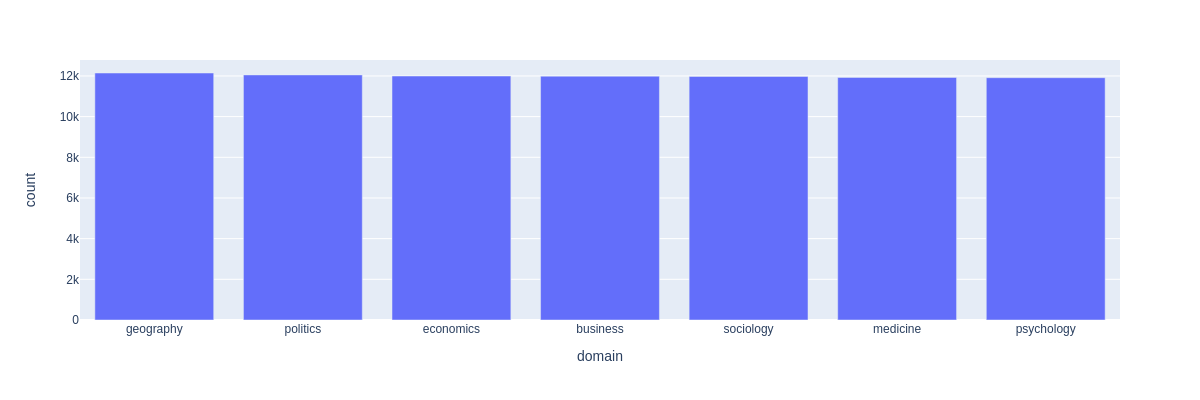
\includegraphics[width=0.5\linewidth]{figures/mag-distribution.png}
    \captionsetup{width=.9\linewidth}
    \caption{Class distribution of the MAG  \cite{wang2019review} dataset's 84000 sentences in its \textit{train} split.}
    \label{fig:mag-distribtion}
\end{figure}

SSC is much larger: it contains over 80 million abstracts. Having more data certainly helps in sampling the term distribution more accurately; nonetheless, the law of diminishing returns applies, especially when using simple models. Therefore, the data will be randomly downsampled to give us a more manageable couple of hundreds of megabytes of abstracts. We can see the distribution of class labels in Figure \ref{fig:ss-distribution}. The dataset is considerably less balanced: \textit{medicine} is by far the most voluminous field.

\begin{figure}
    \centering
    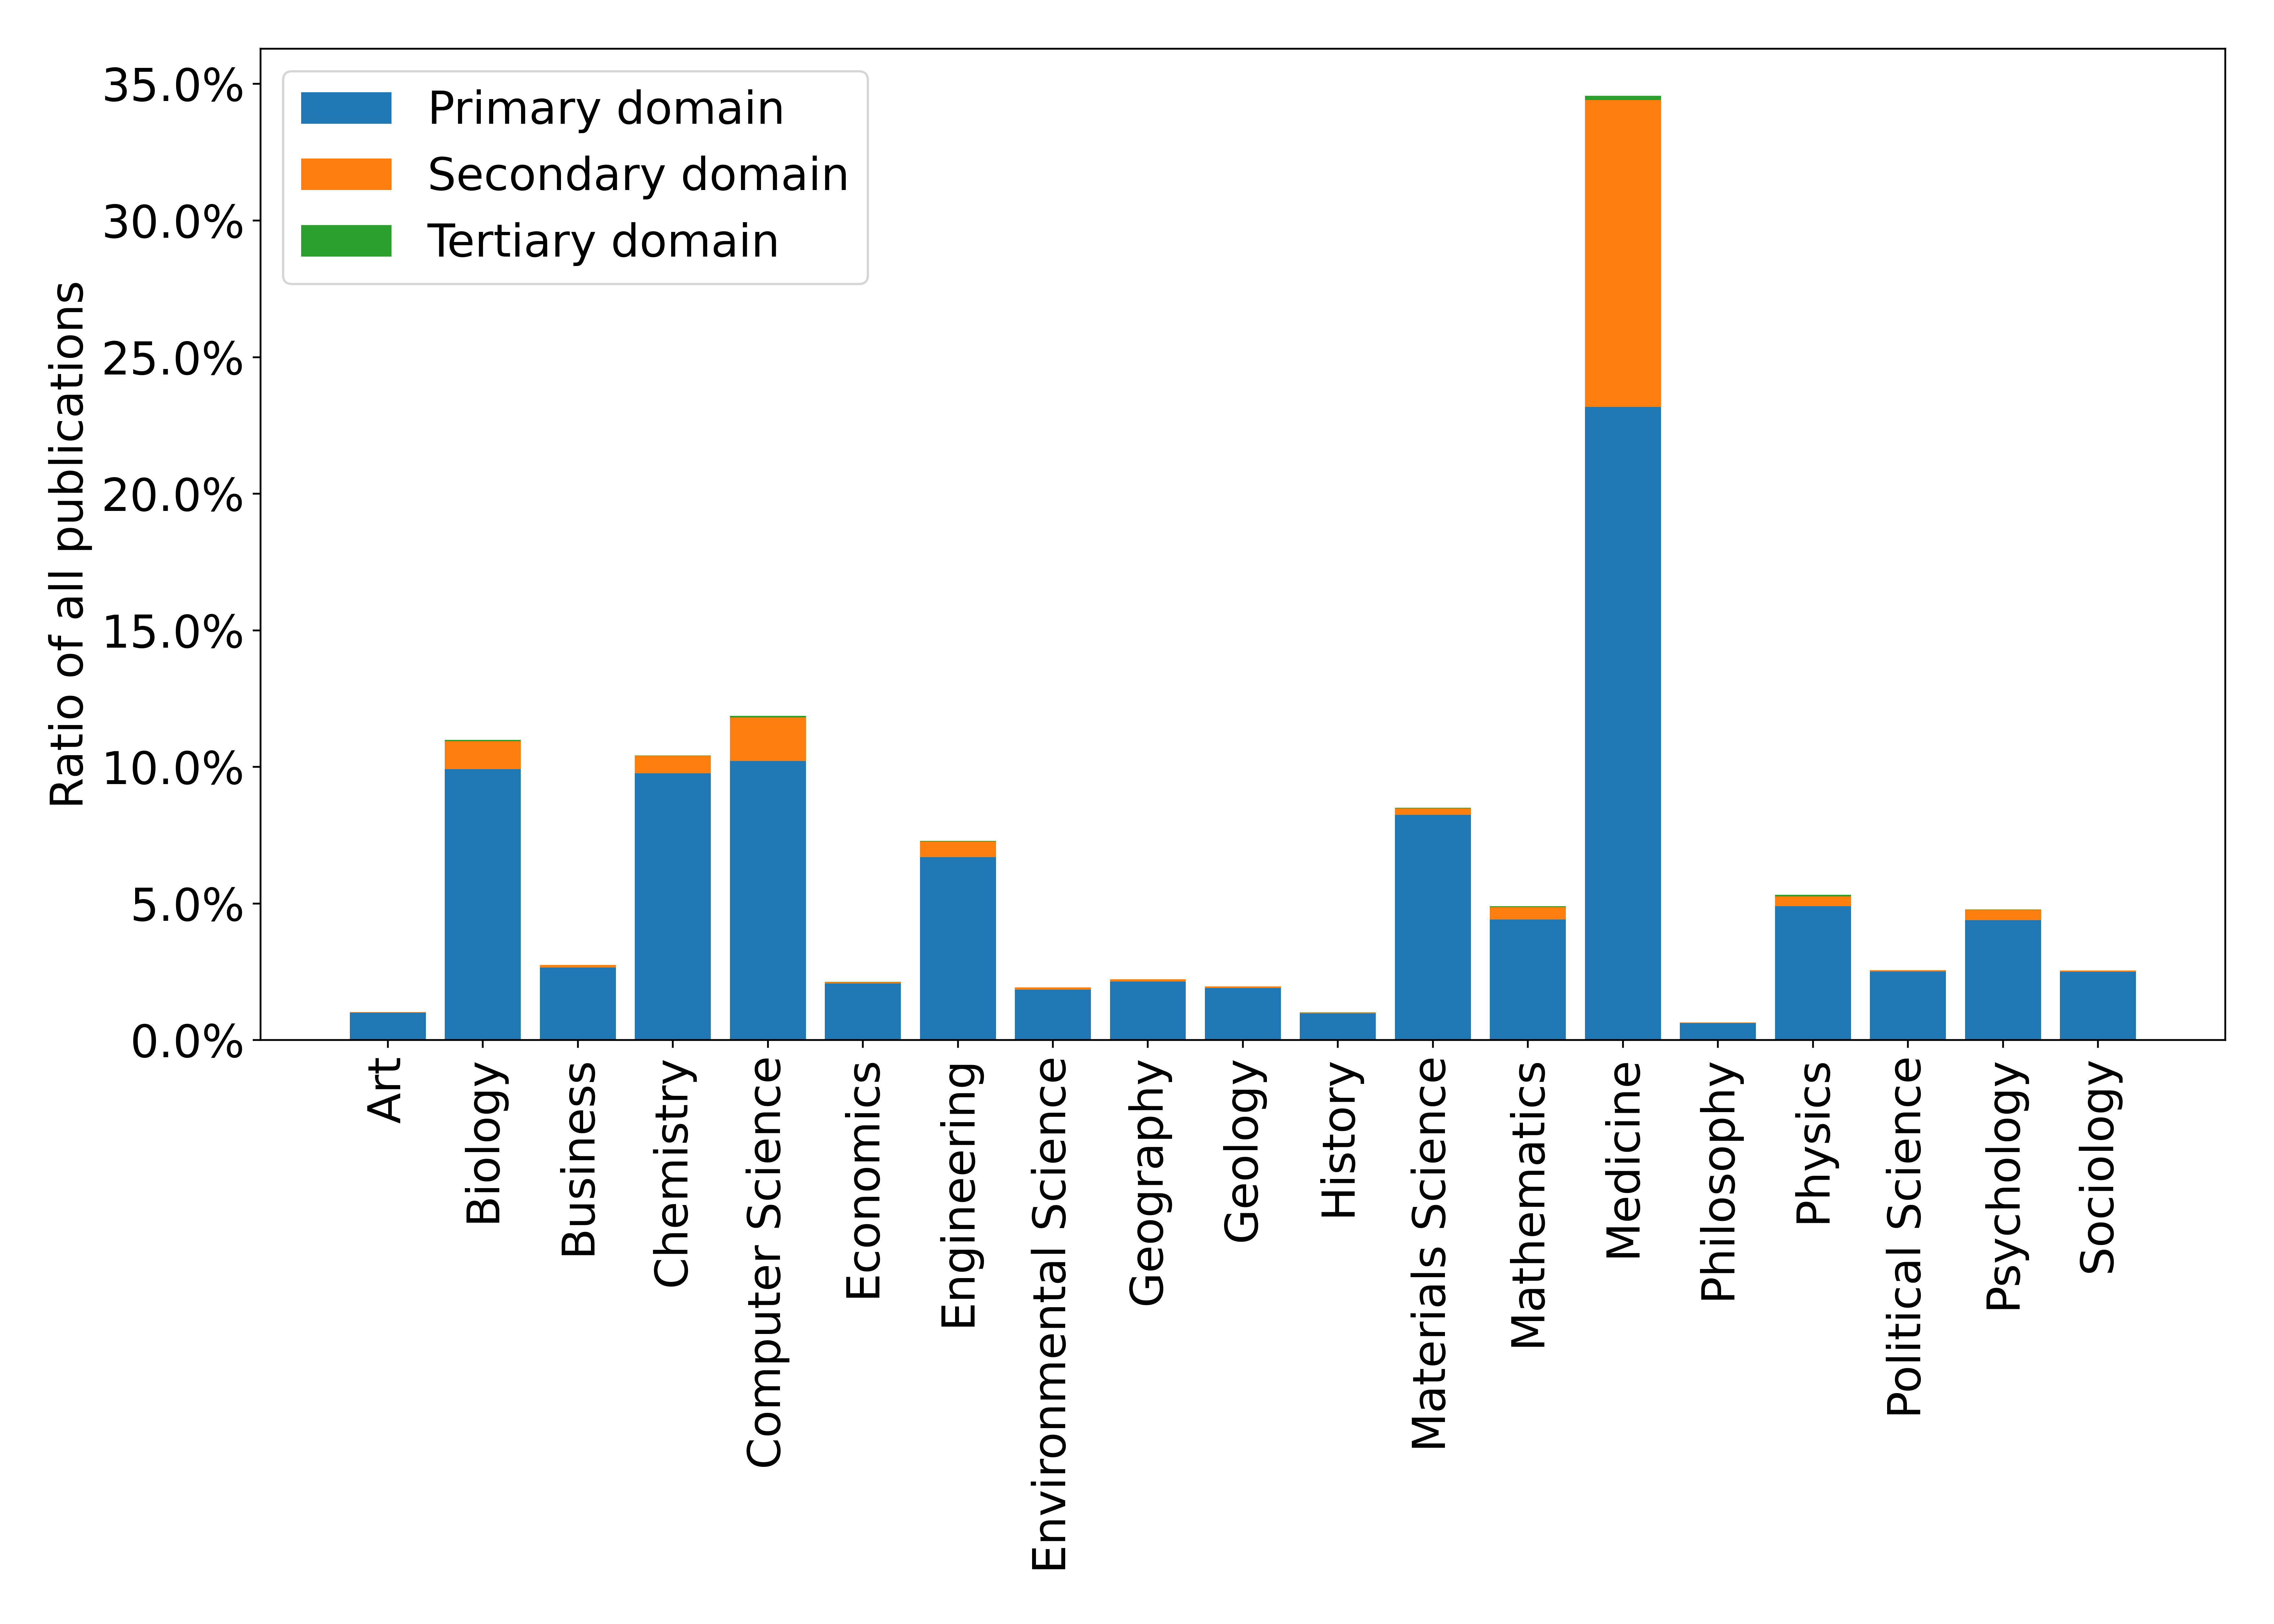
\includegraphics[width=0.8\linewidth]{figures/ss-distribution.png}
    \captionsetup{width=.9\linewidth}
    \caption{Label distribution of the Semantic Scholar dataset \cite{Lo2020S2ORCTS}. Each publication may be assigned at most three domains.}
    \label{fig:ss-distribution}
\end{figure}

\begin{displayquote}
\textbf{Where should we store this data?} ``On my machine'' seems like an easy answer. However, if we have a team working with the data or it has intrinsic value, it must be stored in an easy-to-access, potentially redundant way. Serban et al. \cite{serban2020adoption} expressed this need in the following best practice: \textit{Make Data Sets Available on Shared Infrastructure (private or public)}. Meanwhile, wherever data is stored, it should also be versioned to satisfy the next best practice: \textit{Use Versioning for Data, Model, Configurations, and Training Scripts}.
\end{displayquote}

MAG needs no further preprocessing if we aim to match SciBERT's setup \cite{beltagy2019scibert}. However, since SSC contains heaps of metadata, the relevant parts have to be extracted and preprocessed. In this case, these are the concatenation of the abstract's text and the paper's title along with the paper's domains (there can be multiple domains for a single paper: it is a multi-label classification task). Lastly, the non-English entries are discarded because we only expect to process papers in English.

\begin{displayquote}
\textbf{How should we preprocess the data?} These simple processing steps (filter, map, project) are almost always present in the data science lifecycle. For example, cleaning the input text from various HTML, OCR, PDF, or \LaTeX \hskip 0.12cm extraction artifacts is almost always necessary for text analysis. This is captured in the \href{https://se-ml.github.io/practices}{AI best practices collection} under the following category: \textit{Write Reusable Scripts for Data Cleaning and Merging}. Also, the best practice of \textit{Test all Feature Extraction Code} is somewhat applicable: the applied processing steps must not introduce unwanted artifacts.
\end{displayquote}

\subsection{Methods}

Our aims are twofold: (1) to evaluate a sentence classification model on MAG and compare it with prior art; and (2) to retrain and apply this model for classifying publication metadata (including abstracts). This would allow the ScoutinScience platform to select an appropriate processing pipeline which has been trained on a matching vocabulary (and domain) for each publication. 

It seems reasonable that only considering the distribution (frequencies) of individual terms may be sufficient. For testing this hypothesis, a unigram language model (Multinomial Naïve Bayes) is constructed, and its accuracy is compared with SciBERT's. The former definitely aligns with the advice to \textit{Use The Most Efficient Models}.

Using the MNB implementation of scikit-learn \cite{pedregosa2011scikit}, it only took a couple of lines to create, hyperparameter-optimise, and test a text classifier. Including data loading and visualisations, it takes 71 lines of code (LOC) to be more precise. \footnote{The code is available at \href{https://great-ai.scoutinscience.com/tutorial/}{great-ai.scoutinscience.com/tutorial}.} This further proves how simple it is to use standard packages. The code can be considered for satisfying the \textit{Automate Hyper-Parameter Optimisation} best practice since it also implements an automated hyperparameter sweep. 

The sentences are tokenised into words and vectorised with TF-IDF (with logarithmic term frequency) \cite{buckley1985implementation}, the hyperparameters found via 10-fold cross-validation on the \textit{train} split lead to filtering out tokens which occur in fewer than five documents or more than 5\% of the documents.

\begin{displayquote}
\textbf{What could be automated here?} As discussed in Section \ref{section:accessible-ai}, libraries exposing algorithms and even SOTA models can already be considered mature and accessible. In this case, only scikit-learn was utilised, but subjectively, most popular libraries have a similarly easy-to-use API. Therefore, I see no urgent need for further action regarding the \textit{experimentation} step of the lifecycle in connection with the AI best practices.
\end{displayquote}

\subsection{Results \& Discussion}

\begin{figure}
    \centering
    \includegraphics[width=0.8\linewidth]{figures/mag-confusion.png}
    \captionsetup{width=.9\linewidth}
    \caption{Confusion matrix of a Naïve Bayes classifier on the MAG dataset's sentences. The matrix is normalised column-wise. Notice, how most mistakes happen between semantically similar classes, for instance: \textit{politics} -- \textit{sociology} or \textit{business} -- \textit{economics}.}
    \label{fig:mag-confusion}
\end{figure}

\begin{figure}
    \centering
    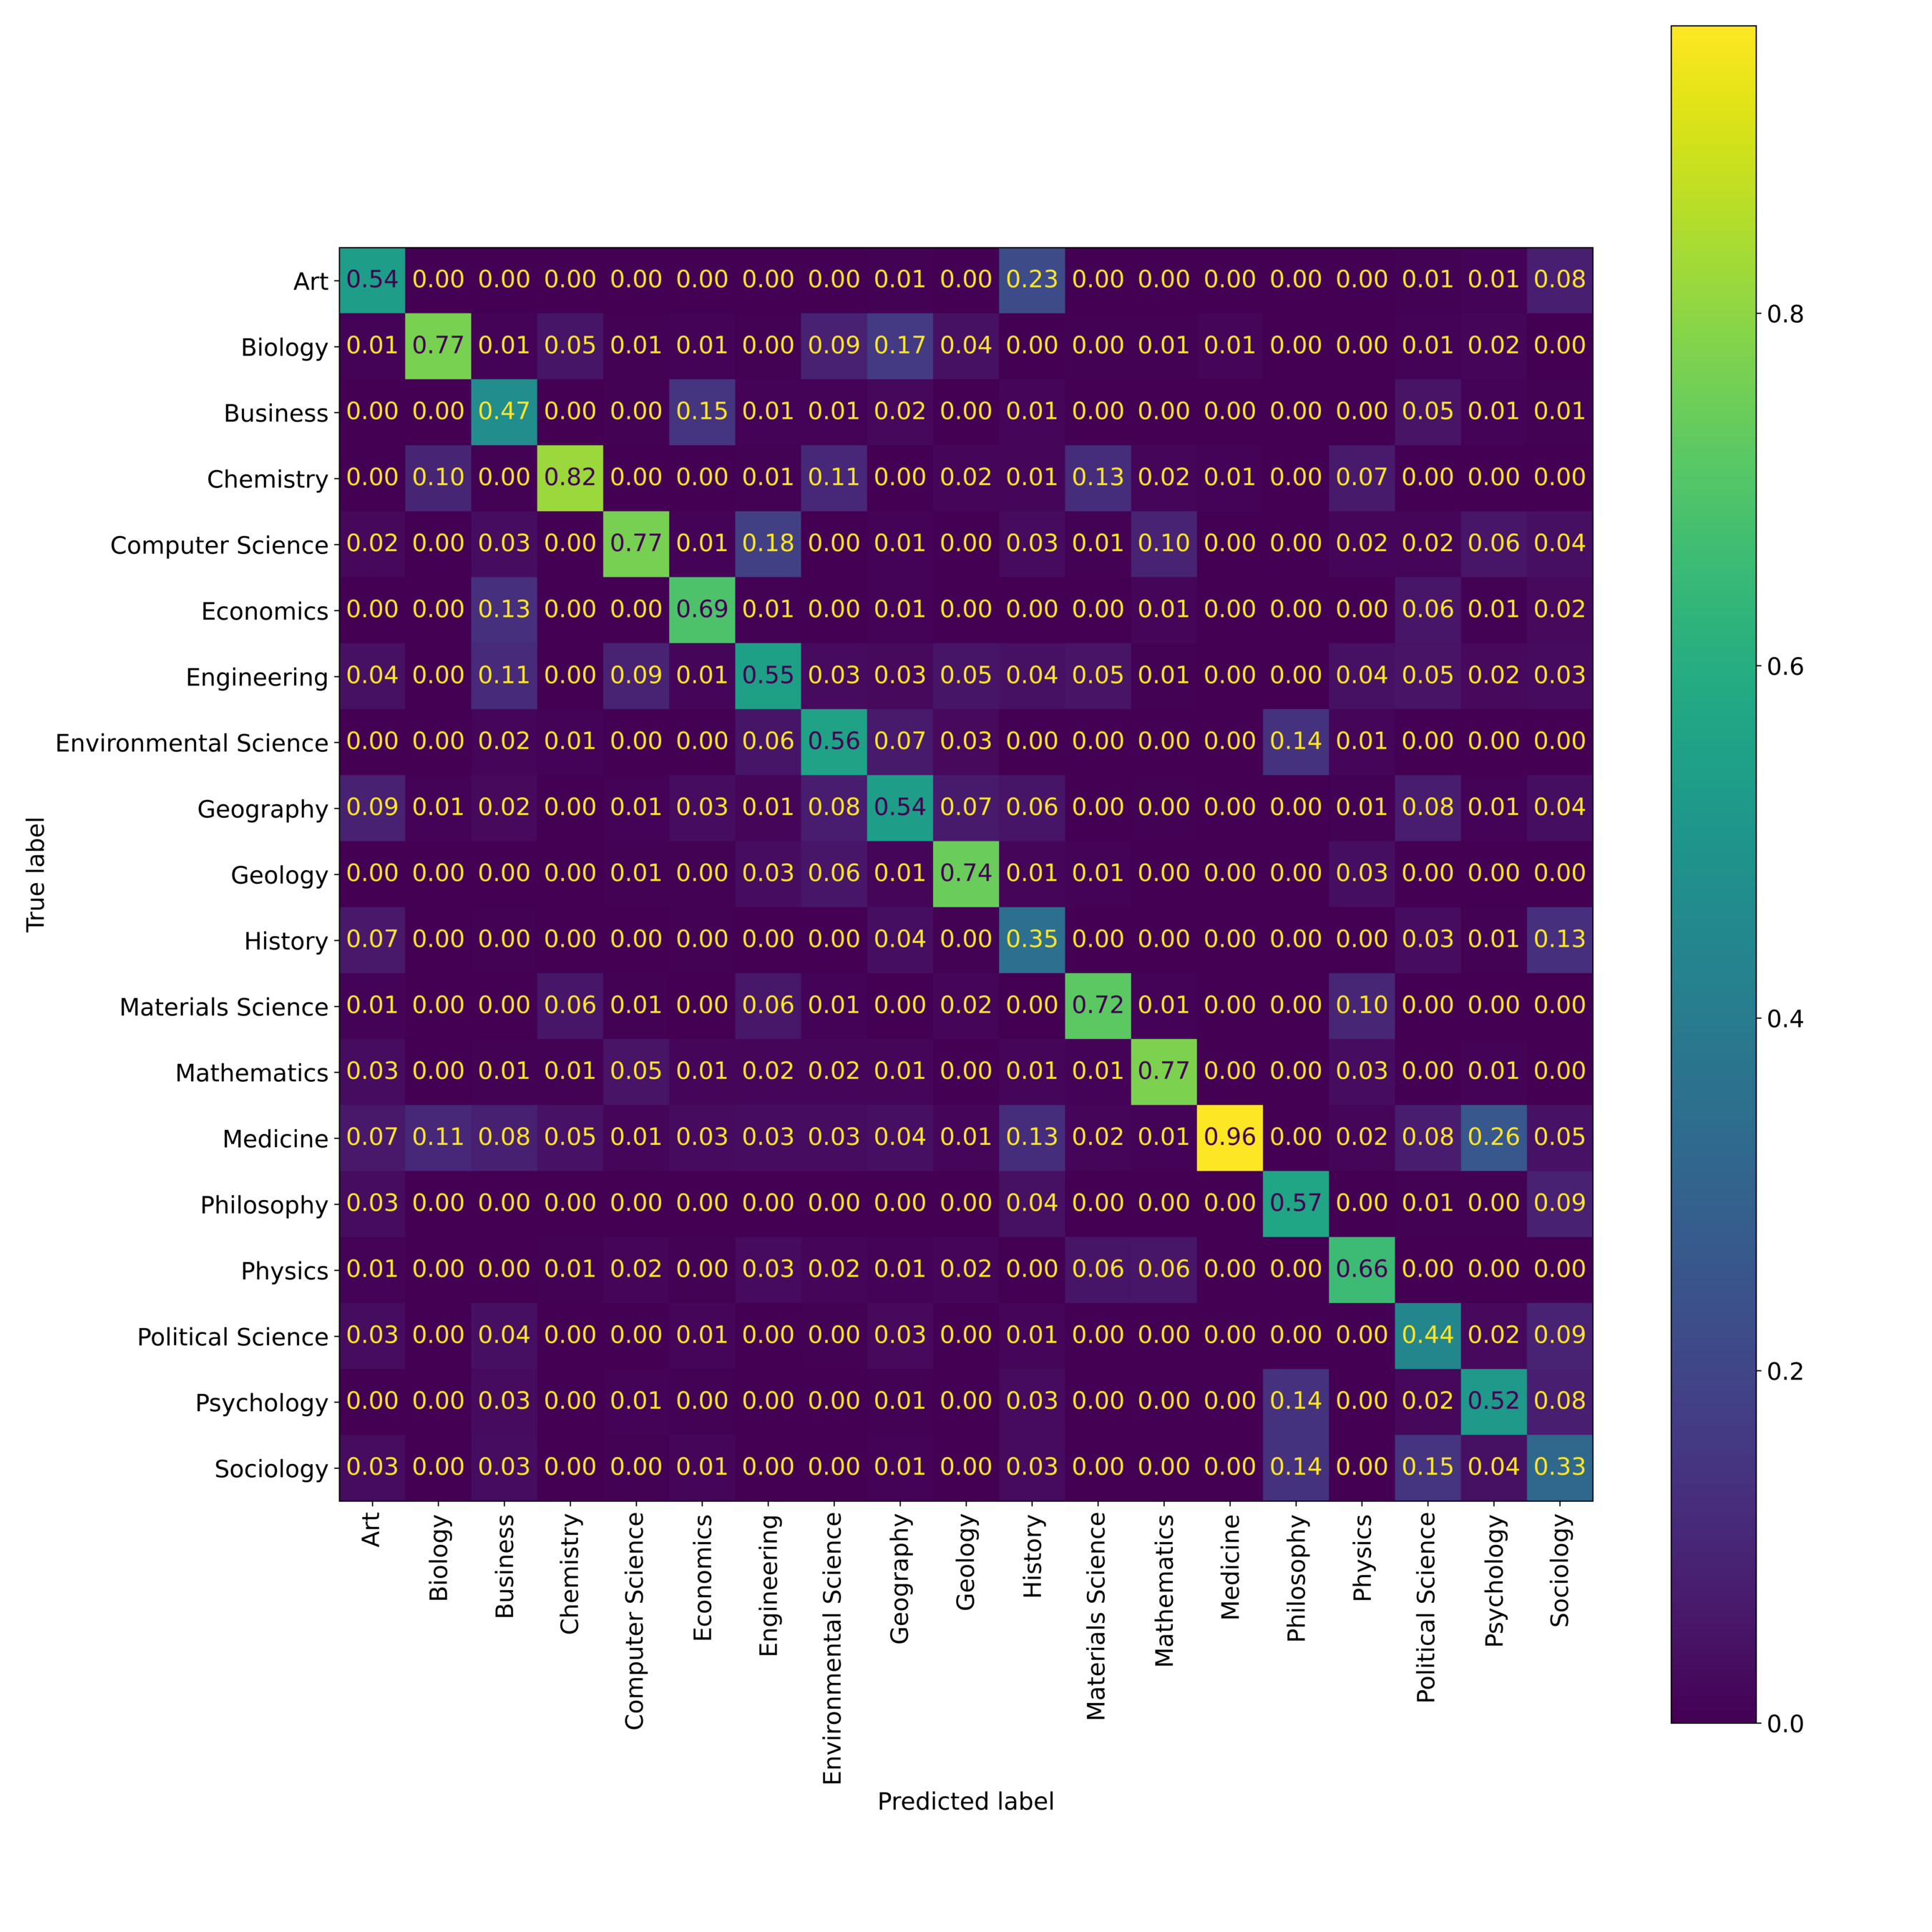
\includegraphics[width=\linewidth]{figures/ss-confusion.png}
    \captionsetup{width=.9\linewidth}
    \caption{Confusion matrix of a Naïve Bayes classifier on the SSC dataset's sentences. The matrix is normalised column-wise. Notice, how most mistakes happen between semantically similar classes, for instance:  \textit{philosohpy} -- \textit{sociology} or \textit{history} -- \textit{art}.}
    \label{fig:ss-confusion}
\end{figure}

When this model is applied to the \textit{test} split of MAG, we get the confusion matrix of Figure \ref{fig:mag-confusion}. This Naïve Bayes classifier achieves a whopping $0.6795$ F1 score. This is $2.3\%$ more than SciBERT's on the same dataset. Thus, it seems that MNB clearly outperforms SciBERT for this particular use case: it is not only more accurate, but its model is magnitudes smaller, while it is also considerably faster to train (or finetune in the case of SciBERT) and use (its running time is in the order of milliseconds per publication). It also has no upper limit on the input length. Thus, this experiment validates choosing MNB for the task over SciBERT.

It is, of course, not entirely surprising that the sophisticated transformer architecture of SciBERT is not necessary for a straightforward task like this. Apart from phrases, the relations between separate words of a sentence do not carry nearly as much discriminative power as the identity of the terms \cite{hand2001idiot}; hence, there is little reason for using an attention mechanism. The fact that SciBERT even works in any way on this task is already a testament to its general applicability. Nevertheless, this short experiment has proved that we can safely opt for using MNB for production.

Since Multinomial Naïve Bayes is best at returning a single label and SSC has multiple labels per datapoint: for evaluation purposes, it is checked whether the returned label is contained in the labels of the ground truth. On this dataset, MNB achieves a lower macro-average F1 score of 0.59.\footnote{The code for this is available at \href{https://great-ai.scoutinscience.com/examples/simple/deploy}{great-ai.scoutinscience.com/examples/simple/deploy}.} The weighted-average F1 is 0.70, and the overall accuracy is also 70\%. The substantial difference between the macro and weighted averages comes from the unbalanced distribution of the labels.

The lower F1 score is not surprising because this dataset has more than twice as many classes. Additionally, the mistakes made are defensible when we look at Figure \ref{fig:ss-confusion}: most of them are between close or related classes.

\begin{displayquote}
This is the usual point where papers conclude: a proof-of-concept/prototype has been built, and its performance demonstrated, measured --- and usually --- explained. Nonetheless, in an industrial setting, our problem is far from being solved: it has yet to be deployed.
\end{displayquote}

\subsection{Deployment}

First, an inference function needs to be written that can take input on the fly and calculate a corresponding prediction. Since we aim to follow the best practices, namely: \textit{Explain Results and Decisions to Users} and \textit{Employ Interpretable Models When Possible}, explaining the results is expected. Fortunately, with our simple model, it is easy to determine the most influential weights, thus, words. The explanations are derived by taking the top 5 tokens from the input text ranked by their feature weights. The last deployment step may be to provide access to our model for others.

\begin{displayquote}
\textbf{How do we provide an interface for the inference function?} We either have an offline or online inference workflow (or both). For the former, we have to provide a way to use it in batch processing; a simple Python function may be adequate for this purpose, though allowing it to be easily (or automatically) parallelised would improve its consumers' DX. If it is an online workflow, we must have a service running continuously and accepting input at any time. This can be achieved by a remote procedure call (RPC) interface or, more commonly, a web API. Developers usually refer to these as REST APIs, and sometimes, they even follow the conventions of REST. Either way, we must develop a wrapper over the service to make it available to other internal/external consumers.
\end{displayquote}

According to the body of research on the adoption of best practices, this is where many real-world projects conclude. This also happens to be \textbf{the gap}. Believing that solely focusing on the research and experiments is good enough is a fallacy: when following this approach, the deployment step ends up being a rushed attempt of wrapping the \textit{AI} and putting it in the production environment. This is, inarguably, a deployment. However, it likely follows very few of the best practices, which can lead to suboptimal real-life performance, lack of accountability, lack of opportunity to improve, and possibly an overall negative societal impact.

\begin{displayquote}
\textbf{How could we implement more best practices?} The most notable missing software/operations features are the lack of automated deployment, automated regression testing, online monitoring, persisting the traces, graceful error-handling, taking feedback on the results (if possible in the use-case), calculating the online accuracy based on the feedback, and retraining the model if necessary using novel data. These all correspond to best practices.
\end{displayquote}

\section{Bridging the gap with GreatAI}

First, let us revisit the library's scope for clarification. As concluded in Section \ref{section:scope}, \textit{GreatAI} should ease the \textit{transition} step between prototypes and production-ready deployments. However, this leaves open the question of what constitutes this step. There are cross-cutting concerns; for example, feature extraction is implemented and used in the training phase, but it is also deployed alongside the model. The robustness criterion has to be met by this procedure even though its implementation is only in focus in the earlier stages of the project. Since having an untested function deployed into production can have severe repercussions, I conclude, assuring its correctness lies within the scope of \textit{GreatAI}.

This section briefly explores how the problems raised can be solved using \textit{GreatAI} and the API it provides to best fit the needs of its users. We first focus on the aspects of data, then we discuss the utility of helper functions, and lastly, the automated wrapping of services.

\subsection{Handling data} \label{subsection:large-file}

The obstacles coming from the intertwined nature of different models are widely recognised \cite{haakman2021ai,amershi2019software,sculley2015hidden}. This can lead to non-monotonic error propagation, meaning that improvements in one part of the system might decrease the overall system quality \cite{amershi2019software}. The importance of schema versioning in an environment of rapidly changing models and transformations is highlighted for a specific use-case in \cite{van2017versioning} and more generally by the \textit{Use Versioning for Data, Model, Configurations and Training Scripts} best practice. These emphasise the requirement for versioning models and, in general, data.

We have to address two kinds of data storage needs: training data and trained models. Because our code is probably already tracked under Git (and \href{https://octoverse.github.com/#lets-look-back-at-the-code-and-communities-built-on-git-hub-this-year}{likely synchronised with GitHub}), using the Git Large File Storage (LFS)\footnote{\href{https://git-lfs.github.com/}{git-lfs.github.com}} might seem intriguing. However, it is a paid (and surprisingly expensive) service of GitHub, especially when we factor in the expected sizes of the models and training data with the fact that the only way to remove files counting towards our quota is to \href{https://docs.github.com/en/repositories/working-with-files/managing-large-files/removing-files-from-git-large-file-storage#git-lfs-objects-in-your-repository}{delete the entire repository}.

An open-source tool, the Data Version Control (DVC)\footnote{\href{https://dvc.org/}{dvc.org}} provides a nearly perfect alternative. It comes with a command-line interface (CLI) inspired by Git's and can be integrated with several backend storage servers. Its only downside is, of course, that it is one more tool that increases the complexity of the project and the initial setup time. If this is an acceptable price to pay, then I personally recommend opting for DVC. Nevertheless, if this may prohibit a team\footnote{As was the case with MLFlow tracking in an ING team described in Section \ref{section:industry}.} from properly handling data according to the best practices, I present a simpler solution.

The complexity of an API can be decreased by relying on its users' preexisting knowledge, and known patterns \cite{hermans2021programmer,ousterhout2018philosophy}. Therefore, we can reuse familiar APIs, such as the \texttt{open()} method from Python. Therefore, a method is proposed which provides the same interface; however, the backing storage can be a mixture of local disk space, S3-compatible storage, MongoDB, or any other storage backend. It provides a superset of \texttt{open()}'s interface\footnote{\href{https://docs.python.org/3/library/functions.html\#open}{docs.python.org/3/library/functions.html\#open}}: the same parameters can be used with it resulting in similar observed behaviour. The expected features: versioning, progress bars, caching, garbage collecting the cache, and automatically deleting old remote versions are all present and come with recommended --- but easy to see and change --- configuration.

Easing development is not merely about automating everything but also about making the code easy to change (which is the \textit{Viscosity} dimension of CDCB). Going from opening a local file on the disk with the built-in open method, to opening a file from S3 is as easy as changing \texttt{open('file.txt', 'w')} to \texttt{LargeFileS3('file.txt', 'w')}. In the case of the latter, an additional \texttt{version} keyword argument can also be given to lock ourselves in using a certain version which is very much desired in the case of models.

\subsection{Utilities}

It is easy to notice multiple recurring tasks when it comes to processing text. Cleaning it from various extraction artifacts and normalising characters is one of the most common. But splitting sentences, language tagging, and robustly lemmatising are also often recurring tasks. Because having reusable and tested feature extraction code covers two best practices, it seems straightforward that a utility module could be created for this, which could be extensively tested through unit testing.

This is exactly the motivation behind \texttt{great\_ai.utilities}. Extra care has to be taken not to overfit these utilities on the cases considered in this chapter; however, I believe these are versatile enough to be helpful in many text-related contexts. A conclusive answer to this assumption will be found during the interviews.

Implementing the unit tests uncovered multiple edge cases and even runtime errors; hence, the merit of \textit{Test all Feature Extraction Code} best practice is unequivocal. There is one more best practice that could be partially covered here, especially because its solution also helps both during batch inference but also at training/feature extraction time: \textit{Enable Parallel Training Experiments}.

A function called \texttt{parallel\_map()} is implemented which closely mimics the API of the built-in Python function: \texttt{map}. Furthermore, it exemplifies how even a close to trivial function can improve the DX by magnitudes. Rooted in the global interpreter lock (GIL)\footnote{\href{https://wiki.python.org/moin/GlobalInterpreterLock}{wiki.python.org/moin/GlobalInterpreterLock}} of CPython, in almost all cases, multi-threading does not lead to higher performance of CPU-bound tasks. For this purpose, multiprocessing has to be used. Fortunately, the built-in \texttt{multiprocessing} library has a great API. However, doing a parallel mapping task with a progress bar still takes about a dozen lines. This can deter people (at least me) from taking advantage of more than just a single CPU core during exploratory experimentation. With \texttt{parallel\_map()}, this challenge becomes a single-line, routine task. 

\subsection{Deployment approach}

Some of the expectations one might have for data-intensive (such as AI) software are similar to that for software in general. These are also captured by the best practices: \textit{Use Continuous Integration}, \textit{Automate Model Deployment}, and \textit{Enable Automatic Roll Backs for Production Model} to name a few. It is important to notice that these have already been solved by software engineering, more specifically, by the DevOps paradigm \cite{leite2019survey}. 
In line with the findings of John et al. \cite{john2020architecting} on the SOTA of AI deployments, I suggest we wrap the applications in a format more compatible with existing DevOps toolkits. Instead of reinventing the wheel, we should rely on more established DevOps best practices for implementing the SE4ML deployment best practices. Besides, organisations are expected to have their deployment processes for classical applications; thus, allowing them to reuse those for AI applications seems to be the most convenient approach.

Based on personal empirical evidence, three types of software artifacts are identified (in the context of Python) for which a wide range of established practices exist. WSGI server\footnote{\href{https://peps.python.org/pep-3333/}{peps.python.org/pep-3333}} compatible applications, executable scripts, and Docker Images\footnote{\href{https://docs.docker.com/registry/spec/manifest-v2-2/}{docs.docker.com/registry/spec/manifest-v2-2}}. To achieve this, \textit{GreatAI} provides a compatibility layer between simple Python inference functions and all the above common artifacts. Taking functions as input for the first step also satisfies the requirement to be \textbf{General}. Nevertheless, to also allow customisation, additional configuration, metadata, and behavioural specification can be given as well.

The main advantage of the wrapping approach is that it does not require any input from the clients (by default). I opted for a decorator \cite{gamma1995design}, which lets users wrap their function by adding a single additional line of code as shown in Listing \ref{listing:hello-world}. After which, the created WSGI application can be accessed through the \texttt{greeter.app} property where \texttt{greeter} is the identifier of the user-defined function. A CLI script (\texttt{great-ai}), along with a \texttt{Dockerfile} are also provided to cover the other two deployment artifacts.

\begin{listing}[!ht]
\begin{minted}[
frame=lines,
framesep=2mm,
baselinestretch=1,
linenos
]{python}
from great_ai import GreatAI

@GreatAI.create
def greeter(name: str) -> str:
    return f"Hello {name}!"
\end{minted}
\captionsetup{width=.9\linewidth}
\caption{Simplest example using \textit{GreatAI} for wrapping a function. In practice, \texttt{greeter} probably would be the inference function of an ML model.}
\label{listing:hello-world}
\end{listing}

Coincidentally, deployment best practices can be easily implemented in this wrapper layer. In the first iteration, these are input validation, persisting traces, online monitoring, and generating documentation. Input validation may be used to \textit{Check that Input Data is Complete, Balanced and Well Distributed}. Traces are essential for both \textit{Log Production Predictions with the Model's Version and Input Data} and \textit{Provide Audit Trails}. However, traces can also indirectly help \textbf{Robustness} because even production systems cannot be expected to be perfect. Saving and letting the users filter on encountered errors while allowing them to correlate those with the inputs producing them is imperative for facilitating debugging. Lastly, monitoring and documentation correspond with helping best practices: \textit{Continuously Monitor the Behaviour of Deployed Models} and \textit{Communicate, Align, and Collaborate With Others} respectively.

To allow customising the service's behaviour to fit different use cases, the default configurations can be overridden by calling some library functions. An example of this can be seen in Listing \ref{listing:complex}, while more details of the semantics can be found in the documentation\footnote{\href{https://great-ai.scoutinscience.com/how-to-guides/create-service/}{great-ai.scoutinscience.com/how-to-guides/create-service}}.

\begin{listing}[!ht]
\begin{minted}[
frame=lines,
framesep=2mm,
baselinestretch=1,
linenos
]{python}
from great_ai import GreatAI, parameter, use_model, log_metric

@GreatAI.create
@parameter('positive_number', validate=lambda n: n > 0)
@use_model('secret-number', version='latest')
def add_to_secret_number(positive_number: int, model: int) -> int:
    """This docstring will be exported as documentation."""
    log_metric('log directly into the Trace', positive_number * 2)
    return secret + positive_number

assert add_number(1).output == 5
\end{minted}
\captionsetup{width=.9\linewidth}
\caption{A simple \textit{GreatAI} service with behavioural customisations. In practice, the function would probably be the inference function for an ML model.}
\label{listing:complex}
\end{listing}

\subsection{Summary}

After implementing some features of the library, it can already be used for deploying the previously discussed domain prediction model. In this case, online prediction is expected; hence, the REST API-based deployment is chosen, which is created by \texttt{GreatAI.create} and packaged in a Docker image. This image can be instantiated by the company's existing DevOps pipeline and cloud infrastructure. In the end, users can see one more tag in the header section of publication evaluations, where they can also see the explanation behind the model's decision as demonstrated in Figure \ref{fig:dashboard-domains}. Let us now explore how it fares in a more complex case.

\begin{figure}
    \centering
    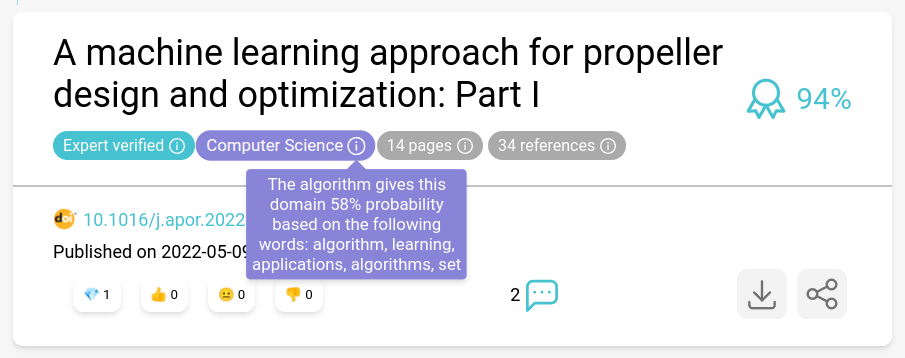
\includegraphics[width=0.7\linewidth]{figures/dashboard-domains.png}
    \captionsetup{width=.9\linewidth}
    \caption{Screenshot of the domain prediction integrated into the ScoutinScience platform, where it is used as a filtering option.}
    \label{fig:dashboard-domains}
\end{figure}

\section{Text summarisation with SciBERT} \label{section:complex-case}

Let us now turn our attention towards a more complex component. The ScoutinScience Dashboard\footnote{\href{https://dashboard.scoutinscience.com/}{dashboard.scoutinscience.com}} contains a full-page evaluation view for academic publications. On this, the known metadata, historical trends about the paper's topics, social media mentions, a PDF viewer showing the document, and other augmentation tools are displayed. One of these is the \textit{Highlights} section, which aims to summarise the paper from a technology-transfer perspective.

The current approach uses a simple heuristic based on a set of phrases selected by business developers and extended by the help of a word2vec model \cite{mikolov2013efficient}. The user feedback deemed this implementation slightly helpful but not adequate for providing an accurate overview. Thus, this is the baseline that I attempt to improve on in this section.

\begin{displayquote}
Compared with Section \ref{section:simple-case}, this time around, the toolset of \textit{GreatAI} is available at our disposal. Hopefully, this will streamline the development and --- especially --- the deployment. Given its arguably higher complexity, the experiment falls closer to industrial use-cases, and hence, can give more accurate feedback on how to further improve the API.
\end{displayquote}

\subsection{Background}

Automatic text summarisation (ATS) is also one of the earliest established tasks of text analysis and boasts numerous promising results \cite{el2021automatic}. Text summarisation is usually divided into extractive and abstractive approaches. Even though the latter can lead to more fluent summaries, it is also prone to hallucinate content that is unfaithful to the input \cite{maynez2020faithfulness}. For this reason, extractive techniques are preferred in this case.

Our problem requires generating a special type of summary: it must only concern a single aspect (tech-transfer) of the document. Aspect-based text summarisation has also seen some progress over the last decades \cite{berkovsky2008aspect,hayashi2021wikiasp} but these methods require concretely defined topics. Unfortunately, \textit{tech-transfer potential} is anything but a clear topic definition.

Numerous discussions and interviews with business developers over the last two years made it clear that there is no universally agreed on definition for it. At least, all of them agree that they know it when they see it. Additionally, most of them agree that they can confidently make a decision at the granularity of sentences. This gives rise to an obvious idea: show the experts something that they can annotate. Because the time of experts is valuable, and relevant sentences are few and far between, extra care needs to be taken to improve the ratio of positive examples in the dataset. The research of Iwatsuki Kenichi on formulaic expressions (FE) \cite{iwatsuki2020evaluation,iwatsuki2021extraction,iwatsuki2021communicative,iwatsuki2022extraction} provides a promising direction to do so. 

A formulaic expression is a phrase with zero or more ``slots'' which when filled appropriately, leads to expressing a certain intent. In the context of scientific texts, an example\footnote{Taken from the ground-truth data available at \href{https://github.com/Alab-NII/FECFevalDataset/blob/master/human_evaluation/background.tsv}{github.com/Alab-NII/FECFevalDataset}.} could be: \texttt{it was not until * that}. The asterisk can be substituted with multiple terms and the intention of this expression is (likely) to describe the \textit{History of the related topics}. Iwatsuki et al. identified a set of 39 intentions, compiled a manually labelled dataset \cite{iwatsuki2020evaluation}, and developed multiple approaches for automatically extracting and classifying formulaic expressions in large corpora \cite{iwatsuki2021communicative,iwatsuki2022extraction}.

\subsection{Methods}

In order to compile a new dataset, experts are asked to judge sentences that passed an \textit{intention check}. This pooling approach is commonly used in the field of information retrieval \cite{schutze2008introduction}. The filtering is expected to sieve out sentences that are probably not relevant from a technology-transfer perspective using Iwatsuki's formulaic expression intention labels. Subsequently, relevance judgements --- in the form of \textit{interesting} or \textit{not interesting} labels --- are gathered for these sentences. This method turns the extractive summarisation into a binary classification task for which a SciBERT model \cite{beltagy2019scibert} can be finetuned. Ultimately, the summaries are derived from sentences that are selected by the classifier trained on the experts' annotations.

We have to note two possible shortcomings of this setup: firstly, we assume the FE intentions are strongly correlated with the sought-after aspect, this may or may not be true. secondly, only the individual relevance of the sentences is considered instead of the overall relevance (utility) of the summary. Nonetheless, it is expected that stemming from the length of the documents and the sparseness of the selected sentences, that any combination of them is likely to have low redundancy.

\subsection{Results}

For the first iteration, 1500 sentences were selected for 2 experts to annotate in a binary fashion according to strict guidelines. An example is shown in Figure \ref{fig:annotator}. Afterwards, for measuring the interrater agreement, Cohen's kappa \cite{cohen1960coefficient} is calculated as shown in Equation \ref{equation:kappa}. Which turns out to be \textbf{0.4310} for the two annotators. This happens to be just above the lower end of \textit{moderate agreement}. However, we have to note that the original quality ranges are often criticised for being too relaxed \cite{mchugh2012interrater}. However, in the case of summarisation, Verberne et al. \cite{verberne2018creating} argue that reasonable end-quality can be reached even when the interrater agreement is relatively low. The ground truth is determined by taking the logical disjunction of the annotations.

\begin{figure}
    \centering
    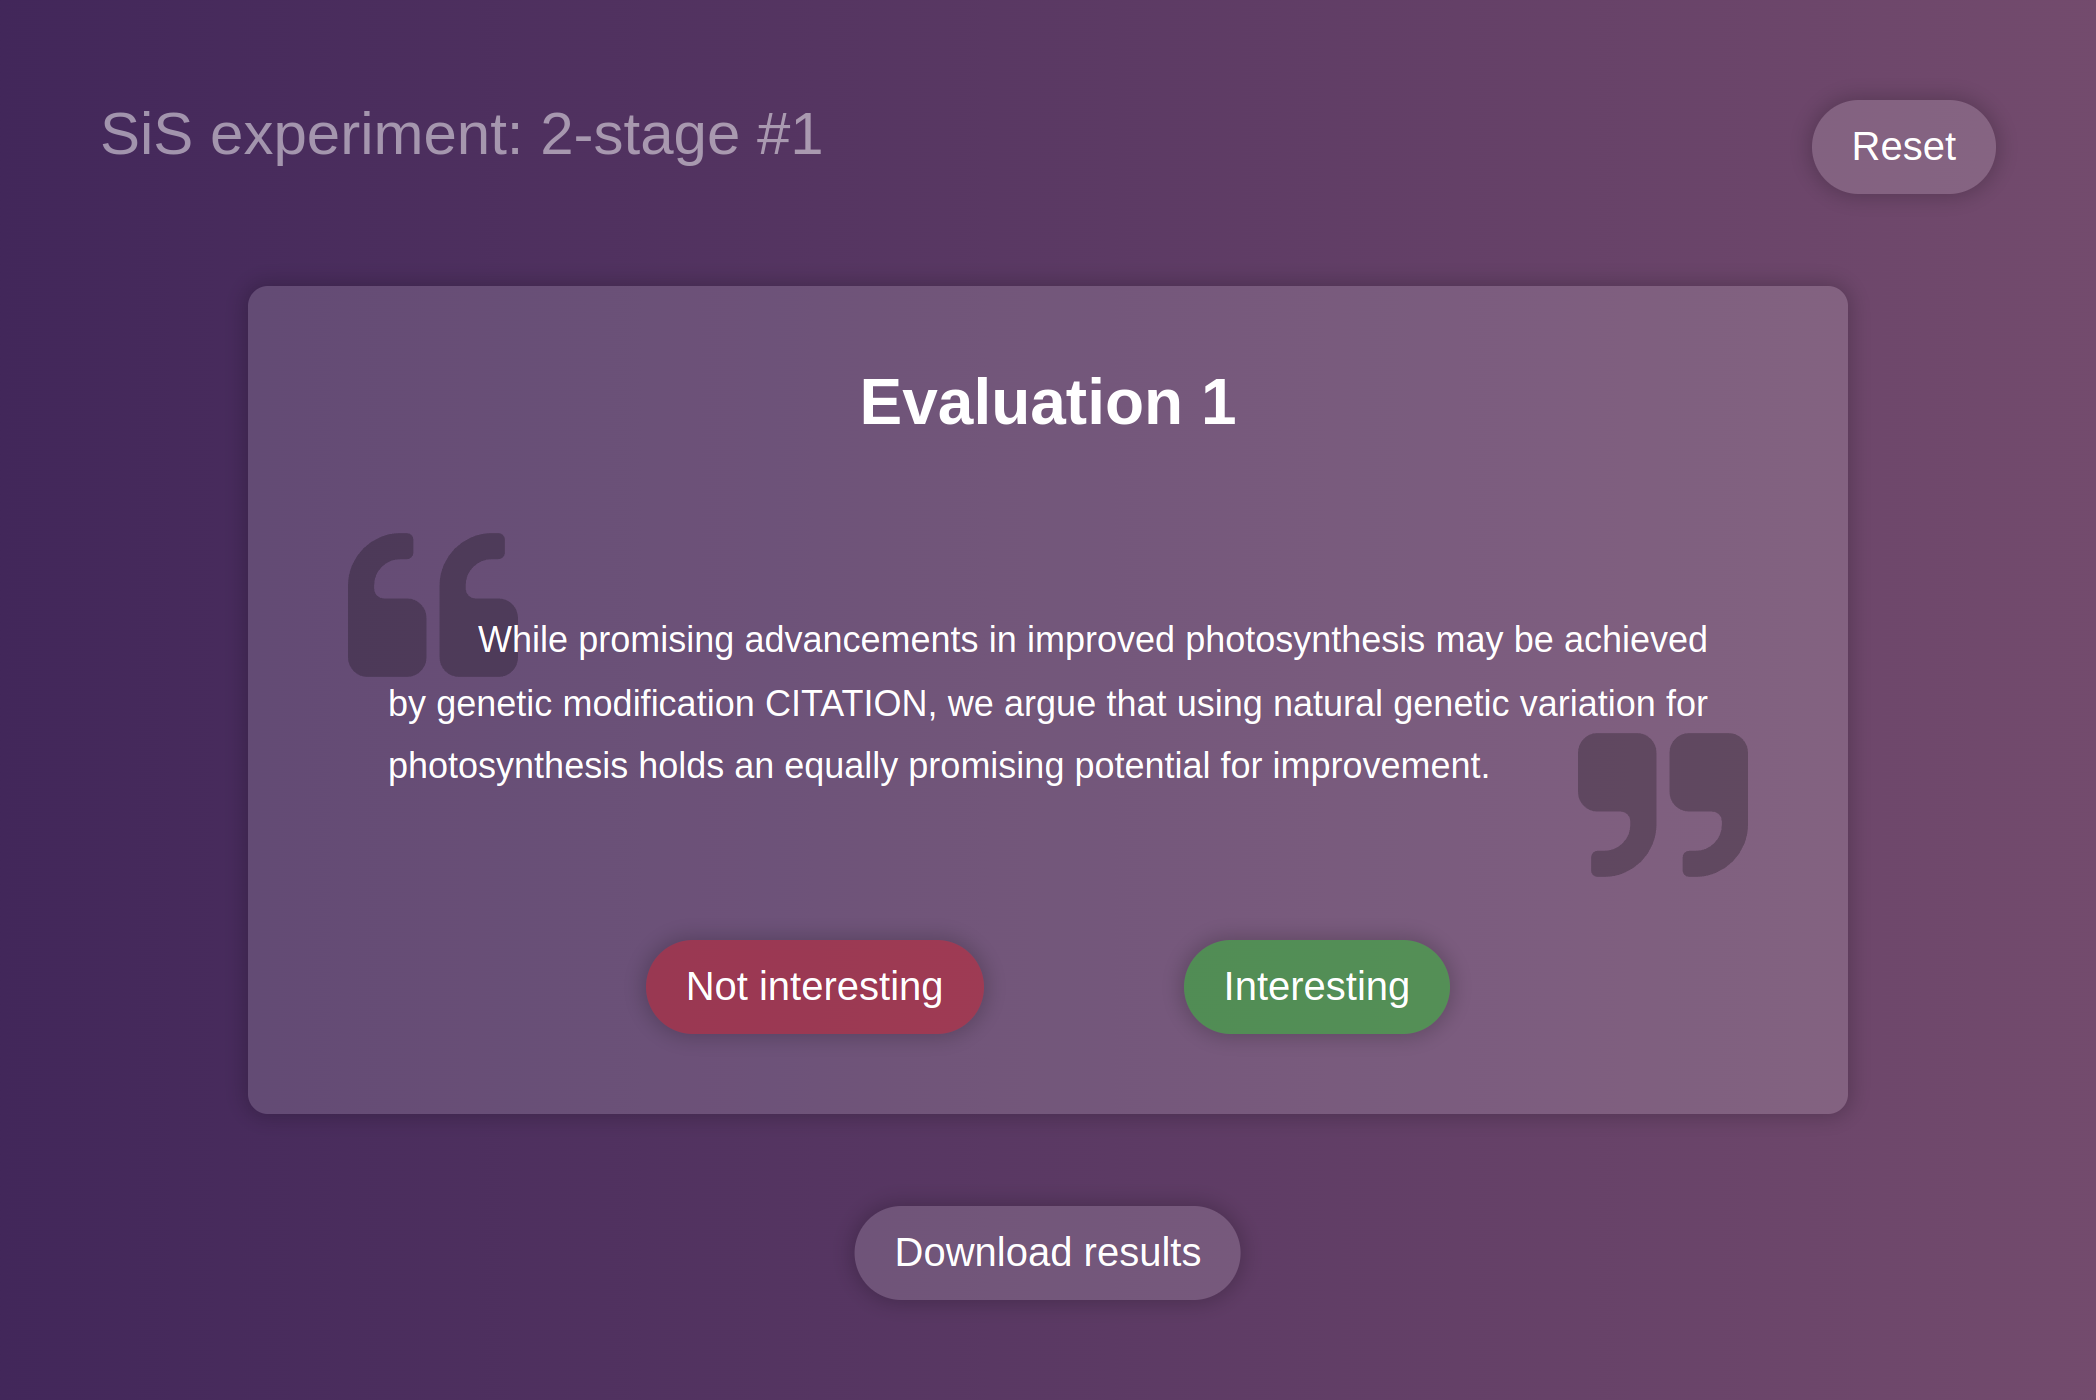
\includegraphics[width=0.75\linewidth]{figures/annotator.png}
    \captionsetup{width=.9\linewidth}
    \caption{Annotator UI showing a single sentence and the two possible labels that can be assigned to it based on its relevance to technology transfer.}
    \label{fig:annotator}
\end{figure}

\begin{equation} \label{equation:kappa}
\kappa_{agreement} \equiv \frac{p_{observed} - p_{expected}}{1 - p_{expected}} = 1 - \frac{1 - p_{observed}}{1 - p_{expected}} 
\end{equation}

The next step is finetuning SciBERT with the help of HuggingFace transformers \cite{wolf2019huggingface}. The data are divided into training and test splits with a ratio of 4:1. From the train split, a validation split is also derived which is used for early stopping. The objective function is the positive class' F1-score and the early stopping patience is 5 epochs. The learning rate is $5 \times 10^{-5}$ and AdamW \cite{loshchilov2017decoupled} is used for optimisation with a weight decay of 0.05. The code can be found in the documentation\footnote{\href{https://great-ai.scoutinscience.com/examples/scibert/train/}{great-ai.scoutinscience.com/examples/scibert/train/}}, it is surprisingly slightly shorter than the code of Section \ref{section:simple-case}.

\begin{displayquote}
\textbf{Reproducability} Reproducible experiments are generally preferred. It is easy to forget to set some seeds values and, for example, end up with different datapoints in the test-train splits during training and validation in a Continuous Integration (CI) pipeline. To facilitate reproducability, it would be useful to reset the seeds of each imported library's random number generators (RNGs) when \textit{GreatAI} is configured. Thus, a feature has been added to detect and reset RNGs of installed and imported libraries. This certainly will not solve the reproducibility crisis \cite{hutson2018artificial} on its own, however, in some cases, it can result in one fewer step to miss.
\end{displayquote}

\begin{displayquote}
\textbf{Utility of LargeFiles} For the purposes of the documentation, the finetuning was conducted in the Google Colab online environment which is excellent for providing anyone with GPU-time for free. However, notebook environments are ephemeral, resulting in the need to manually upload and download all relevant data whenever a new virtual machine (VM) instance is granted. The \texttt{LargeFile} implementation alleviated this problem by handling the uploads and downloads automatically. Of course, first, backwards compatibility had to be solved for Python 3.7 which is the only available environment in Colab.
\end{displayquote}

The best validation results were achieved after 8 epochs which was slightly more than expected but is presumably due to the weight decay. The confusion matrix on the test split can be seen in Figure \ref{fig:scibert-confusion}: regardless the subjective definition of the task, SciBERT manages to achieve good quality which is indicated by an F1-score of \textbf{0.89}.

\begin{figure}
    \centering
    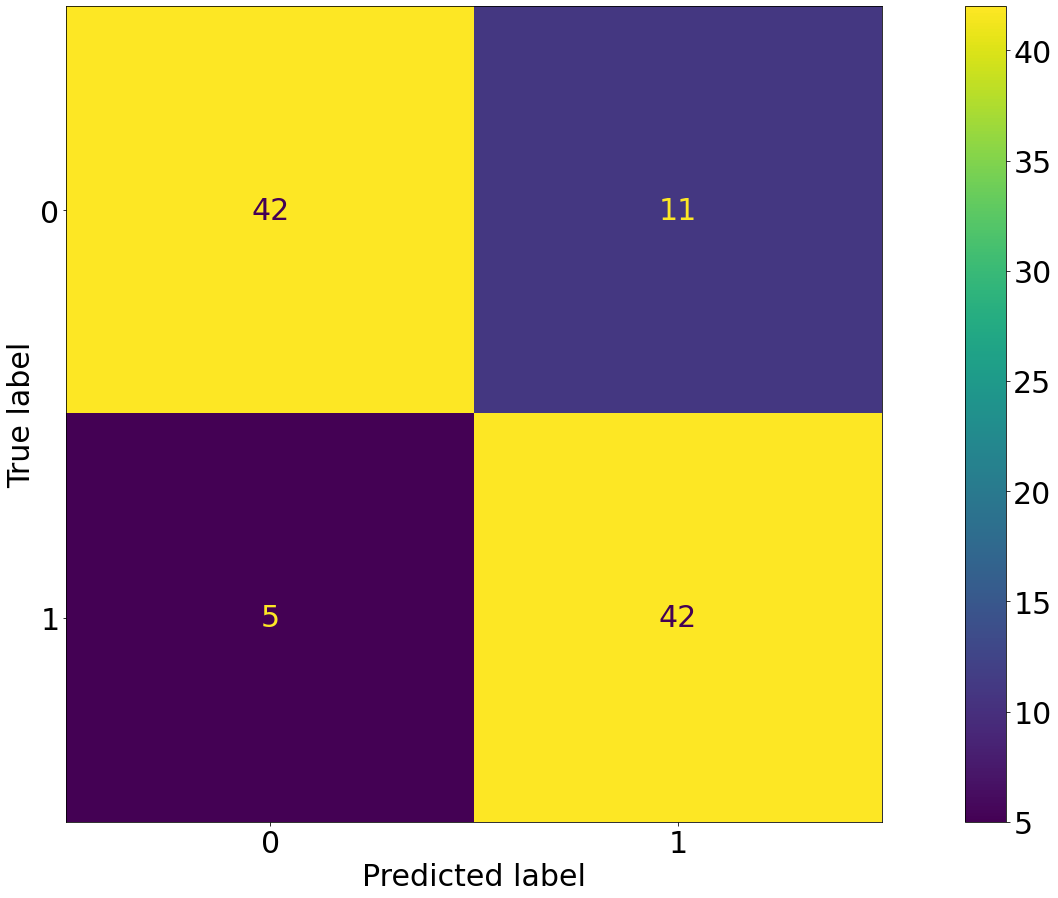
\includegraphics[width=0.4\linewidth]{figures/scibert-confusion.png}
    \captionsetup{width=.9\linewidth}
    \caption{Confusion matrix of the fine-tuned SciBERT model on the \textit{summary candidate sentences} dataset. The values are globally normalised and represent percentages.}
    \label{fig:scibert-confusion}
\end{figure}

Let us check how well the selected sentences correspond with the tech-transfer potential. Users and in-house experts can rate publications (from a tech-transfer perspective) by assigning them to one of four categories: \texttt{A}, \texttt{B}, \texttt{C}, and \texttt{D} with \texttt{A} being the most and \texttt{D} the least promising. This feedback is stored and used for analytic and training purposes. Since both the feedback grade and the ``highlights'' are supposed to reflect the same aspect of papers, therefore, we can reasonably expect some correlation between them.

Figure \ref{fig:histograms} shows the ratio of summary candidate sentences as predicted by the finetuned model in 4 categories (grades) of papers. The two datasets come from non-overlapping sets of papers, hence, the results come solely from the model's ability to generalise. It is interesting to see that the Spearman's rank correlation coefficient \cite{spearman1961proof} between the normalised ``highlights'' counts and the ratings of papers is \textbf{0.4784} and is statistically significant ($P = 5.4 \times 10^{-74}$). This proves the presence of a monotonic association. For context, the correlation between the grades and the number of sentences found by the baseline approach is 0.06597 ($P = 0.03$). We can conclude that the classifier's output is indicative of the publications' tech-transfer potential. 

\begin{figure}
    \centering
    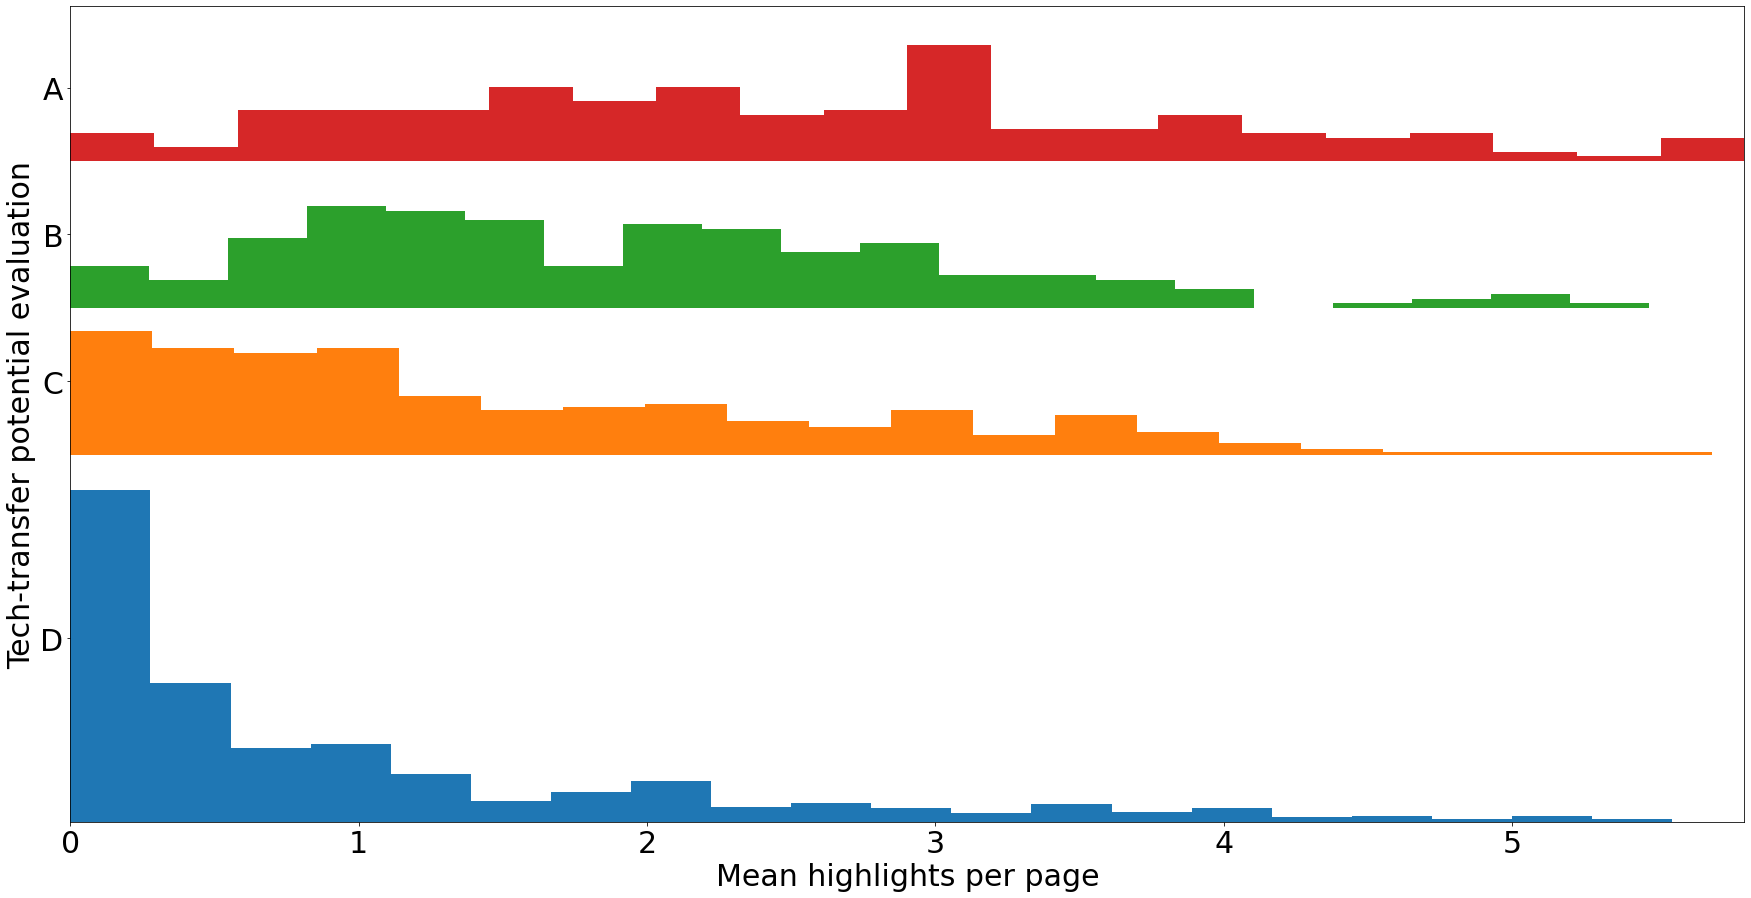
\includegraphics[width=0.85\linewidth]{figures/highlights-histograms.png}
    \captionsetup{width=.9\linewidth}
    \caption{Distribution of mean predicted summary candidate sentence counts in 4 categories. Category \texttt{A} correspond to the most, while \texttt{D} to the least interesting papers based on mean user feedback. The sample size is 1406 (\texttt{D}=715, \texttt{C}=309, \texttt{B}=198, \texttt{A}=184). The histograms are on the same scale.}
    \label{fig:histograms}
\end{figure}

\subsection{Deployment}

To implement the summarisation, at most the top 7 selected sentences are chosen as ranked by their log-probabilities. They are subsequently reordered according to their position in the text. As a quasi-explanation, the tokens' attention scores are visualised and overlaid on the highlighted sentences. The \textit{i}-th token's visualised attention comes from summing up the attention weights of each of the last layer's heads between the \texttt{[CLS]} and the \textit{i}-th token. To improve the end-user experience, a high-pass filter and a stop-word list is applied to the scores in order not to highlight the syntax-related tokens (punctuation, determiners). The service --- after being integrated into the dashboard --- can be seen in Figure \ref{fig:dashboard-highlights}.

\begin{displayquote}
In order to get insights into their inner workings, HuggingFace models can be given \texttt{output\_attentions=True} in their constructor which results in a new property becoming accessible on the results for querying the attentions. The only issue with it is that it is a 5-dimensional matrix which makes exploring and understanding it non-obvious. In short, it has very low \textit{Discoveribility}. For example, the attentions for the UI are calculated with this expression:
\begin{minted}[
baselinestretch=1,
]{python}
np.sum(result.attentions[-1].numpy()[0], axis=0)[0][1:-1]
\end{minted}
Even though the operation is conceptually simple, because of the opaque datastructure, this is anything but obvious to comprehend. Therefore, it is clear that this needs to be avoided in my library design; it has to have a clear and discoverable API which can be achieved by the use of typehints, descriptive property names, and docstrings.
\end{displayquote}

\begin{figure}
    \centering
    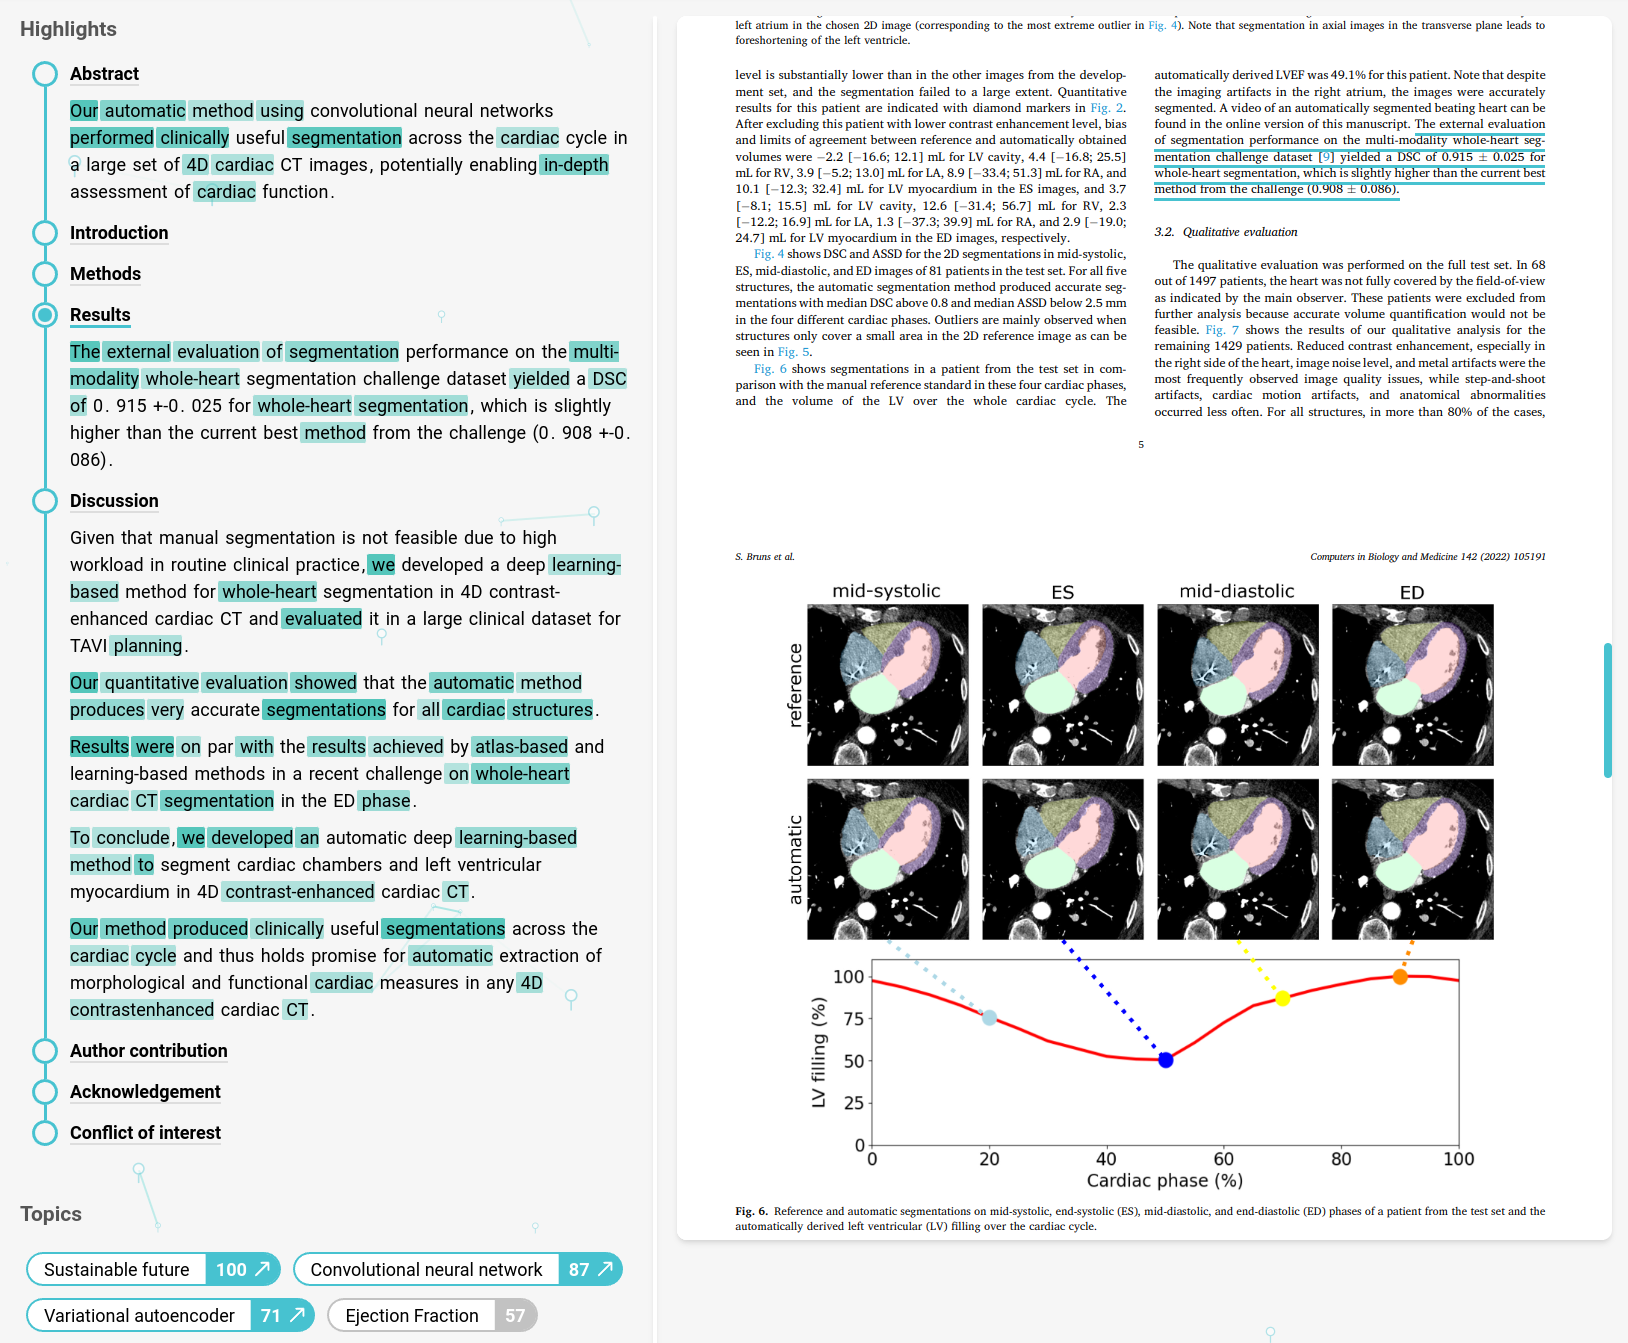
\includegraphics[width=1\linewidth]{figures/dashboard-highlights.png}
    \captionsetup{width=.9\linewidth}
    \caption{The tech-transfer summary of an academic publication (\cite{bruns2022deep}). The titles and sentences can be clicked for navigating the paper on the right, meanwhile some explanation is provided by the highlighted words, the opacity of which corresponds to their attention weights.}
    \label{fig:dashboard-highlights}
\end{figure}

\section{Improving GreatAI}

After having solved two problems by implementing two standalone services and integrating them into an existing ecosystem while relying on \textit{GreatAI} as a primary tool, a wide variety of insights have been gained. In the next couple of subsections, the extra features and design decisions are presented that have been motivated by the \textit{Highlights service}. After which, the final surface of the API is described and evaluated by its relation to the SE4ML \cite{serban2020adoption,serban2021practices} and AI engineering \cite{john2020architecting,john2020ai} best practices.

\subsection{Caching}

Sustainability is an increasingly crucial concern of ethical AI \cite{van2021sustainable}. Without discussing the pros and cons of the green computing movement \cite{10.1145/1400181.1400186}, we can still agree that computing time should not be wasted. To this end, caching the results of expensive operations has to be considered in any AI deployment. In this case, the \textit{Highlights service} is often called multiple times from different other services with the same parameters. With each operation taking up to a couple of seconds, implementing caching can lead to vastly faster response times and an overall more socially conscious deployment.

\subsection{Revisiting \texttt{parallel\_map}}

Even though most inference functions are CPU-bound, turns out, sometimes they involve IO, especially, when relying on the results of other, remote models. This means that a significant performance improvement can be achieved by implementing some inference functions asynchronously \cite{tilkov2010node}. Thus, \textit{GreatAI} also has to support decorating both regular (synchronous) and asynchronous functions. There is one notable consequence of this: the batch processing feature also has to be compatible with \texttt{async} inference functions. Batch processing is still a useful feature since it is likely that async inference functions are both IO (remote calls) and CPU (local evaluation) constrained at the same time, thus, they can benefit from multi-core parallelisation. 

However, the standard library's \texttt{multiprocessing}, the third party \texttt{multiprocess} \cite{mckerns2012building}, and, another popular library, \texttt{joblib}\footnote{\href{https://joblib.readthedocs.io/en/latest/}{joblib.readthedocs.io/en/latest}} all lack the support for efficiently parallelising async functions. For this reason, \texttt{parallel\_map} is reimplemented to create an event-loop in each worker process to keep the efficiency of non-blocking IO while also providing parallelisation for the CPU-bound sections of code.

\subsection{Programmatic integration}

Apart from supporting \texttt{async} calls, there are a couple of more step that can be taken to help integrating any service with a \textit{GreatAI} deployment. This is implemented by the \texttt{call\_remote\_great\_ai} function which hides the networking required to call a \textit{GreatAI} instance's REST API. It takes care of validation, automatic retries, serialisation, and deserialisation. This comes with the added benefit of encouraging decoupled services because the friction of integrating them is no longer noticeable which is beneficial for human collaboration \cite{hasselbring2002component}.

Additionally, a REST API is generated with its accompanying OpenAPI schema\footnote{\href{https://swagger.io/specification}{swagger.io/specification}} and served with a \href{https://swagger.io/}{Swagger} template. It also contains metadata about the function, for instance, its docstring, version, and version of its registered models concatenated in order to be SemVer\footnote{\href{https://semver.org/}{semver.org}} compatible. These can be seen in Figure \ref{fig:greatai-api}. This, combined with a \texttt{/version} HTTP endpoint for programmatic access and validation of the service's metadata proved to be key features when integrating the \textit{Highlights service} into ScoutinScience's service-based architecture.

\begin{figure}
    \centering
    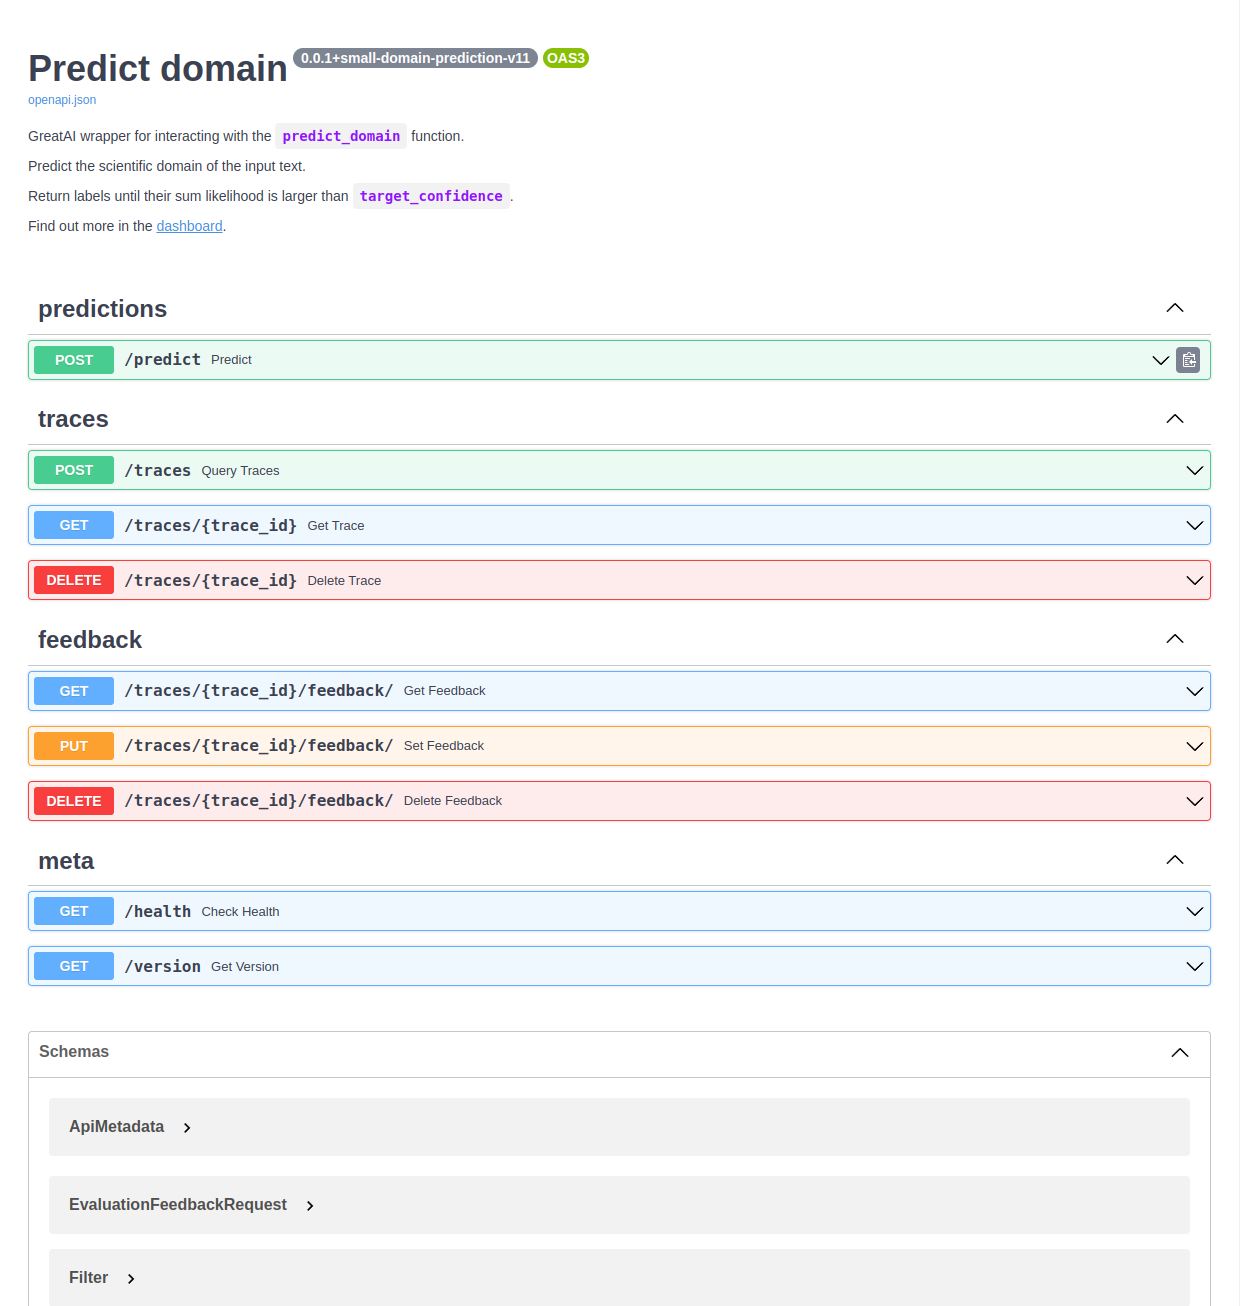
\includegraphics[width=0.85\linewidth]{figures/greatai-api.png}
    \captionsetup{width=.9\linewidth}
    \caption{Documentation of the automatically scaffolded REST API of a \textit{GreatAI} service. Notice, how its version string includes its registered models in a SemVer compliant way: \texttt{0.0.1+small-domain-prediction-v11}.}
    \label{fig:greatai-api}
\end{figure}

\subsection{\textit{Human} integration}

Even though the REST API of \textit{GreatAI} services exposes all necessary features\footnote{Such as providing feedback per prediction, complexly filtering and sorting traces, create-read-update-delete (CRUD) operations for the feedback and traces, accessing live monitoring info (current configuration, versions, cache statistics), etc.} which are great for programmatic access, these are not ideal for direct human comprehension. In order to ease the introduction of \textit{GreatAI} services, a rudimentary dashboard is --- optionally --- generated next to the REST API. The dashboard's main features can be observed in Figures \ref{fig:greatai-header}, \ref{fig:greatai-table}, and \ref{fig:greatai-parallel}. The diagrams and filterable/sortable table are interconnected and are automatically updated, the reactive behaviour is provided by the Dash framework \cite{shammamah_hossain-proc-scipy-2019}.

\begin{figure}
    \centering
    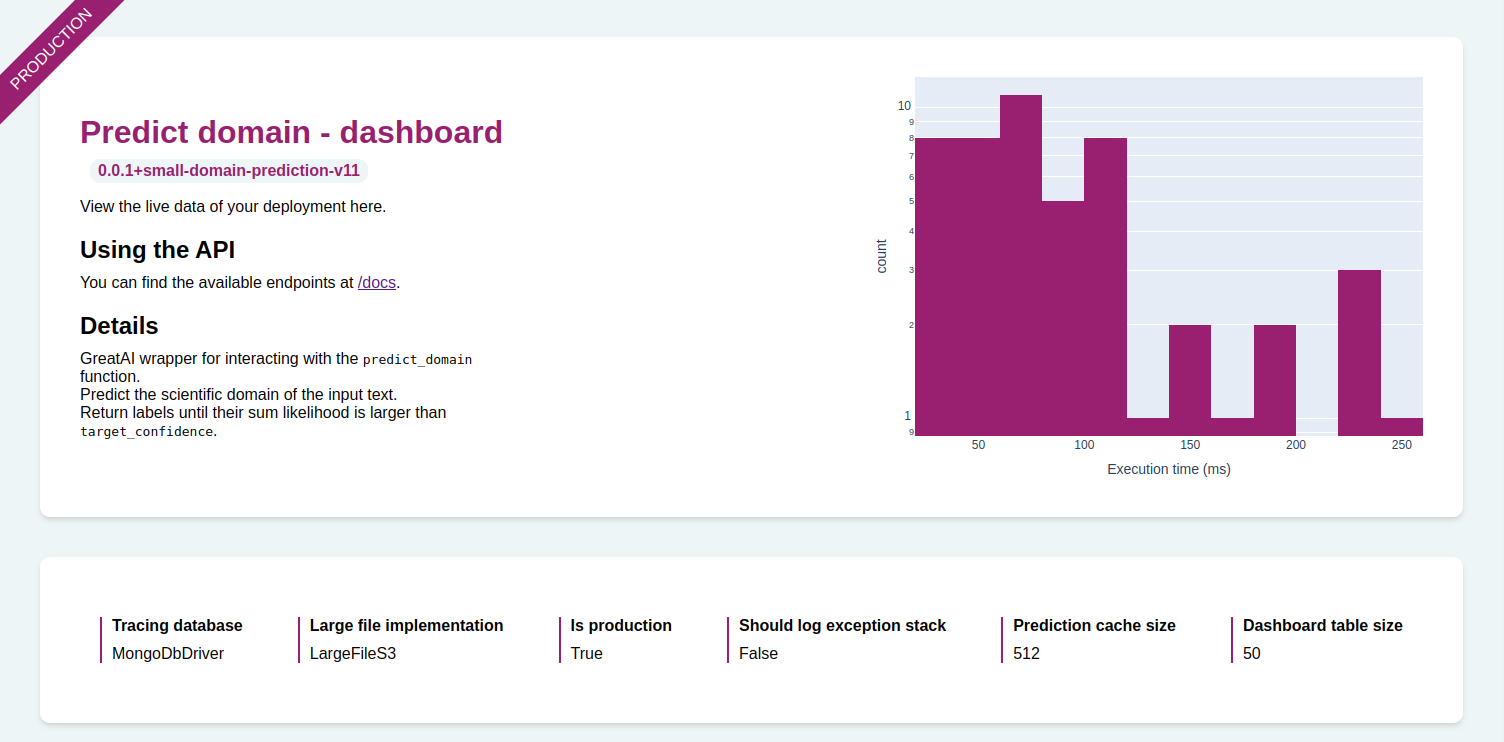
\includegraphics[width=1\linewidth]{figures/greatai-header.png}
    \captionsetup{width=.9\linewidth}
    \caption{The header of the automatically generated dashboard of the service from Section \ref{section:simple-case}. A documentation is generated on the left, while the histogram of response times is shown on the right. The current configuration is prominently displayed on the bottom.}
    \label{fig:greatai-header}
\end{figure}

\begin{figure}
    \centering
    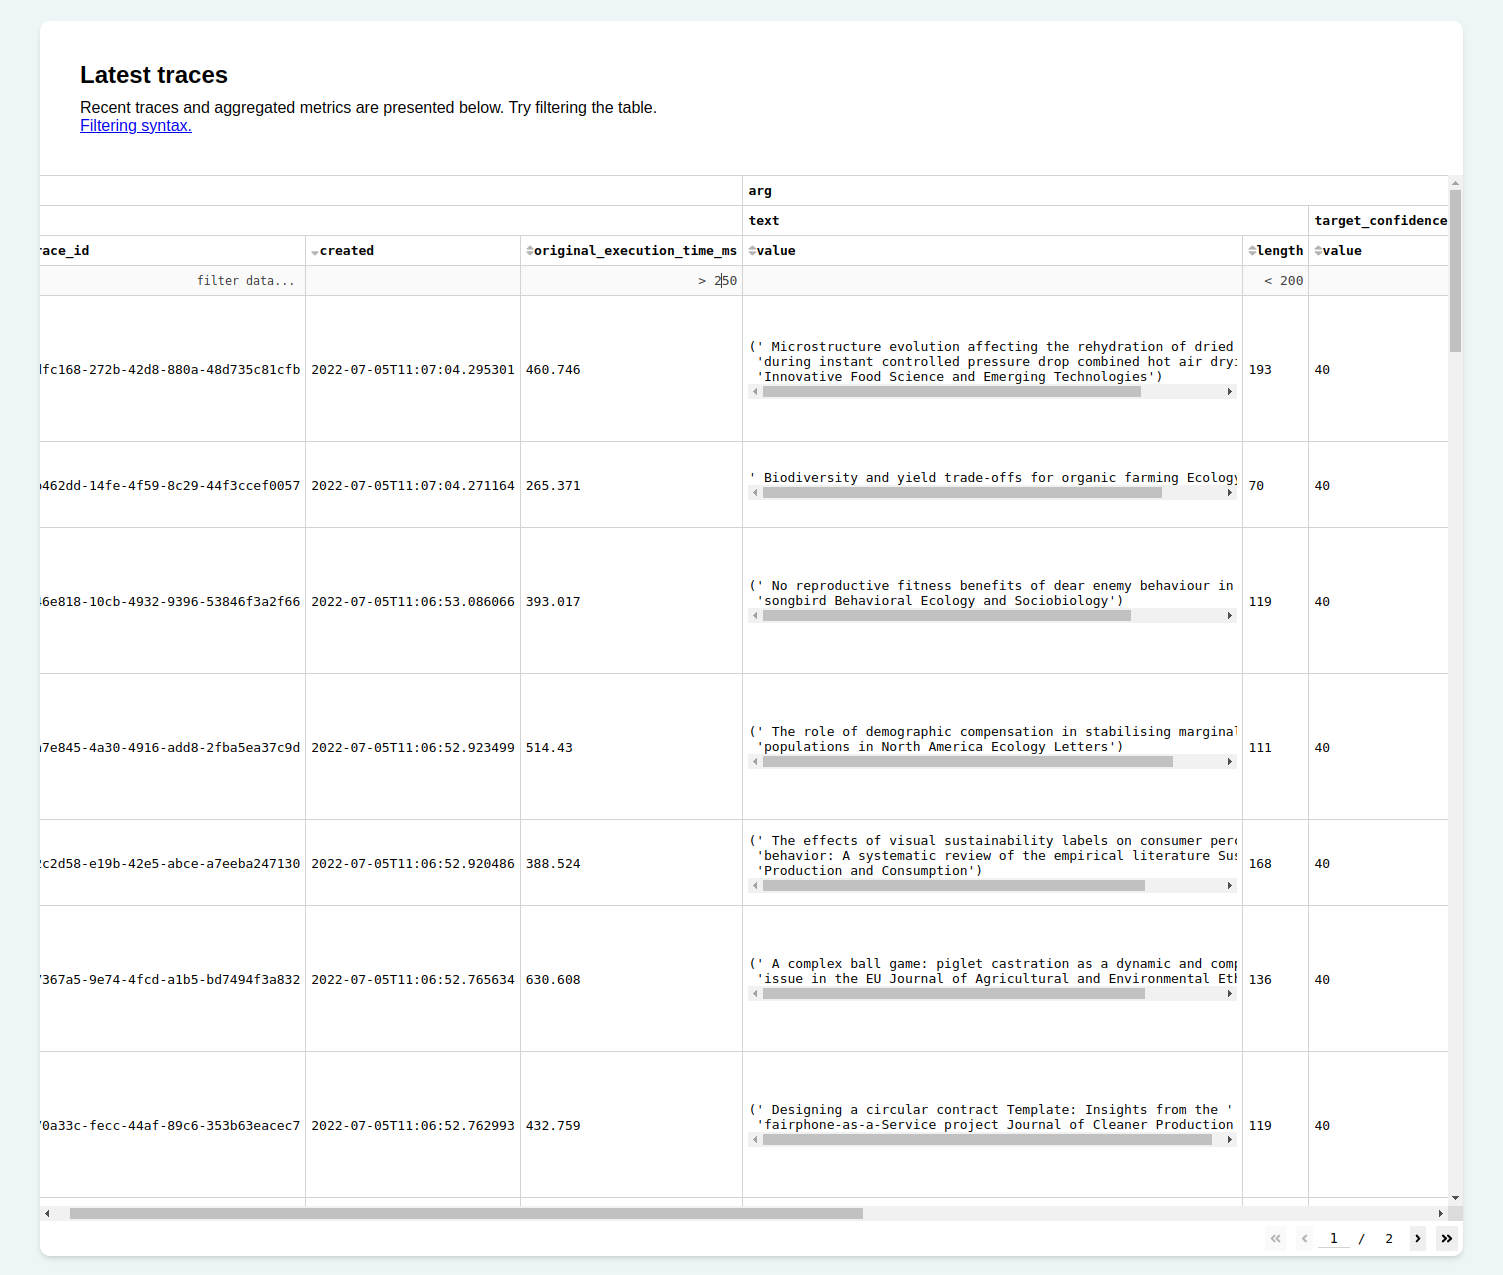
\includegraphics[width=1\textwidth]{figures/greatai-table.png}
    \captionsetup{width=.9\linewidth}
    \caption{A dynamically updating, tabular view of traces matching a user-defined filter. Useful for exploring historical predictions or debugging the cause of exceptions (which are also searchable). The filters set in the table affect the other diagrams of the dashboard.}
    \label{fig:greatai-table}
\end{figure}

\begin{figure}
    \centering
    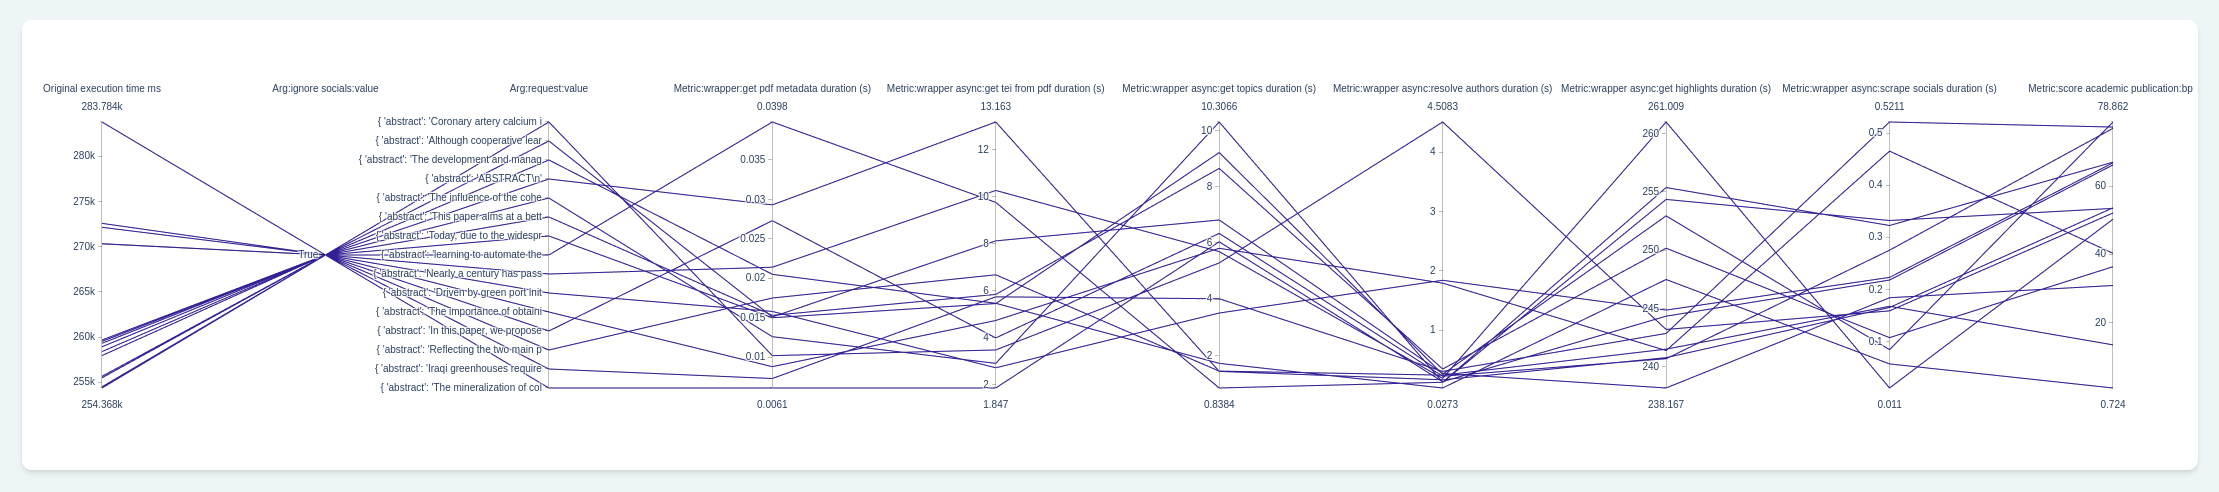
\includegraphics[width=1\textwidth]{figures/greatai-parallel.png}
    \captionsetup{width=.9\linewidth}
    \caption{A parallel coordinates view of the traces displayed in the table above. Adding new axes is as easy as calling \texttt{log\_metric} inside the inference function.}
    \label{fig:greatai-parallel}
\end{figure}

